\section{Numerical results}
\label{sec:results}
In three subsections below, we analyze  the sensitivity of each of the three QoIs. In the first subsection, we discuss  further the probabilistic distribution of the uncertain parameters.  

\subsection{Parameter distribution}
\label{sec:param_sampling}

We now revisit our assumption that all the uncertain parameters are independent and uniformly distributed within $\pm 10\%$ of  their nominal value. We do so by conducting a study of the steady state solutions, i..e, we solve the ODE system (\ref{caboodle}) {\sl without} stimuli as this significantly speeds up computation; indeed, a similar study on the full dynamics proved to not be computationally feasible.  

While parameters are likely to be correlated, we do not know the correlation structure a priori. The model is run, with no stimulus applied, for 919 different parameter samples. Of these 919 runs, 670 of them fail due to ode15s terminating prematurely because its time steps became too small. The remaining 249 yields 139 solutions which the radius reaches a stable steady state (at least for the duration of the time integration) and 110 solutions for which the radius reaches a steady state but subsequently because transient. The left panel of Figure~\ref{steady_states} displays four representative solutions for the radius; the red curves remain in steady state for the duration of our time integration whereas the black curves revert into a transit regime after some time in or near steady state. The right panel of Figure~\ref{steady_states} displays the samples for two parameters (in the buffer equation) which are highly influential in determining the behavior of the solution. A blue * indicates a sample where the solver terminated prematurely, a yellow + indicates a sample where an unstable steady state was observed, a red $\circ$ indicates a sample where the solution remained in steady state. A strong correlation determining the behavior of the solution is observed.

\begin{figure}[h]
\centering
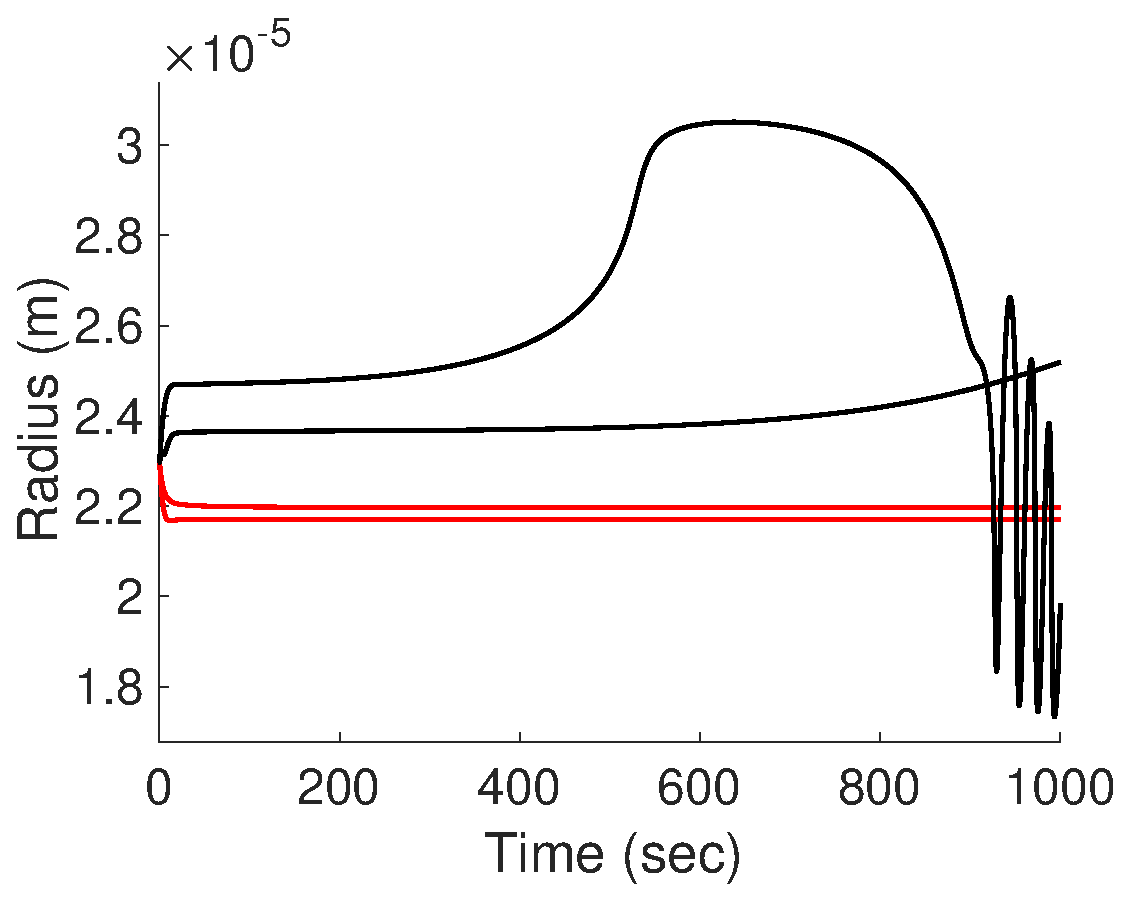
\includegraphics[width=.4 \textwidth]{Figures/Steady_State_Curves.eps}
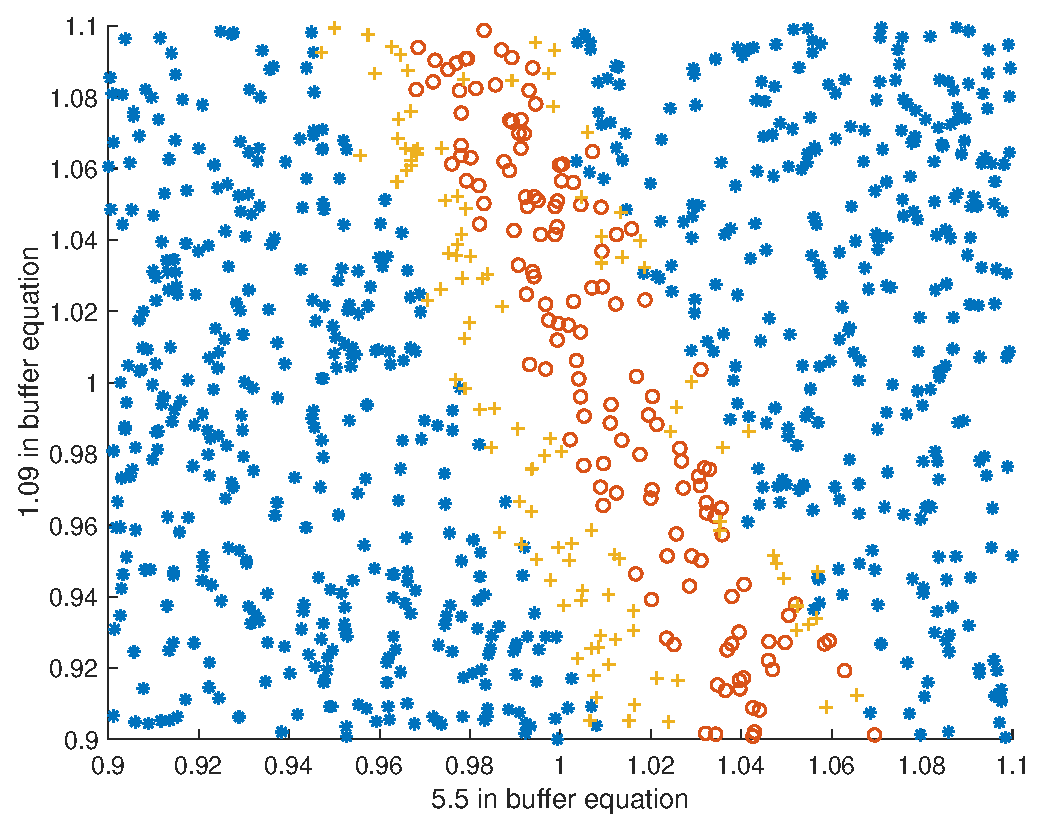
\includegraphics[width=.4 \textwidth]{Figures/First_Iteration_Samples.eps}
\caption{Left: examples of stable (red) and unstable (black) steady state solutions. Right: samples of the buffer parameters using uniform independent sampling. A blue \* indicates the sample yielded a premature termination of the solver, a yellow + indicates the sample yielded an unstable steady state, a red $\circ$ indicates the sample yielded a stable steady state.}
\label{steady_states}
\end{figure}

Observing this correlation, we use the samples for which the radius remained in steady state to fit the two buffer parameters with a bivariate distribution with beta marginals and a Frank copula. The experiment was repeat by sampling the two correlated parameters with the bivariate distribution and all other parameter from their original uniform distributions. The samples yielding steady state solutions where collected, a bivariate distribution fit to them, and the experimented was repeated. After three additional iterations of this process we were able to generate 902 out of 960 samples which yielded solutions with stable steady states (51 solutions had unstable steady states and 7 had premature solver terminations). This fitted distribution is used for all subsequent analysis. 

Samples are drawn and the model, with a stimulus applied (in two separate cases, the 10 second rectangular pulse and the 16 second stimulus from experimental data), is run for each sample. This results in solutions exhibiting three different physiological regimes; they are displayed in Figure~\ref{solution_regimes} where the radius is plotted as a function of time. The leftmost panel corresponds to the typical case when the radius increases in response to the stimulus and then decreases when it is removed; the center panel corresponds to an atypical case where the radius has an initial decrease in response to the stimulus; the right panel corresponds to another atypical case where the radius reaches another steady state an does not decrease after the stimulus is removed.

\begin{figure}[h]
\centering
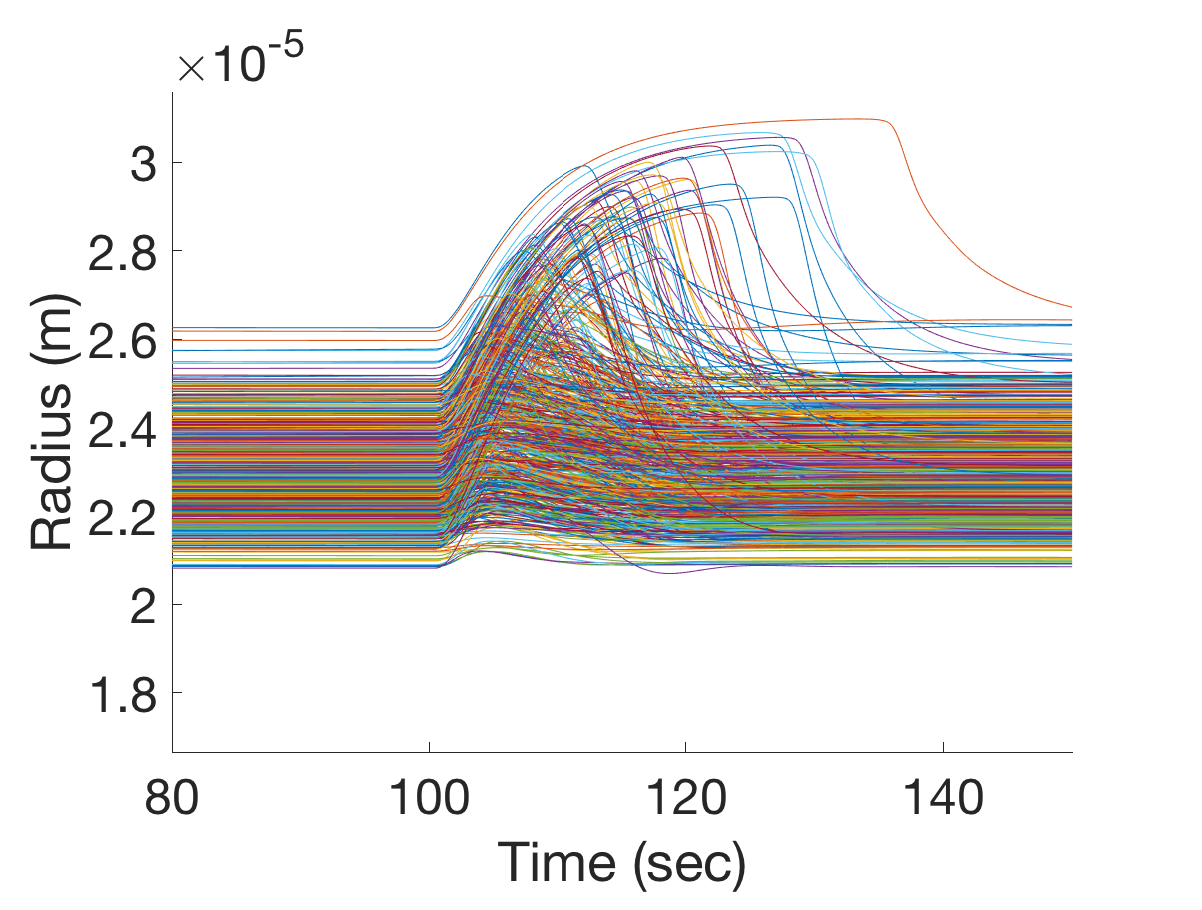
\includegraphics[width=.3 \textwidth]{Figures/Increase_with_Stim_Curves.eps}
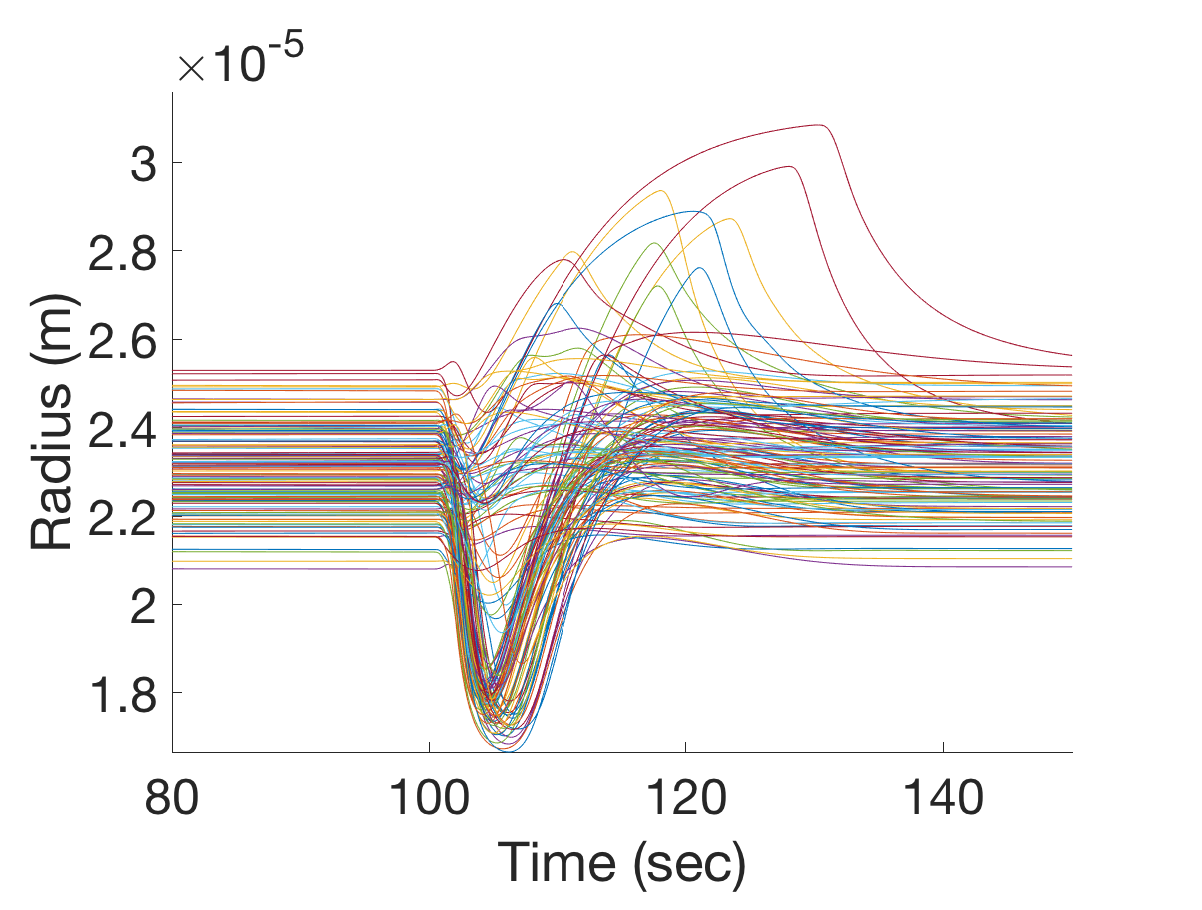
\includegraphics[width=.3 \textwidth]{Figures/Decrease_with_Stim_Curves.eps}
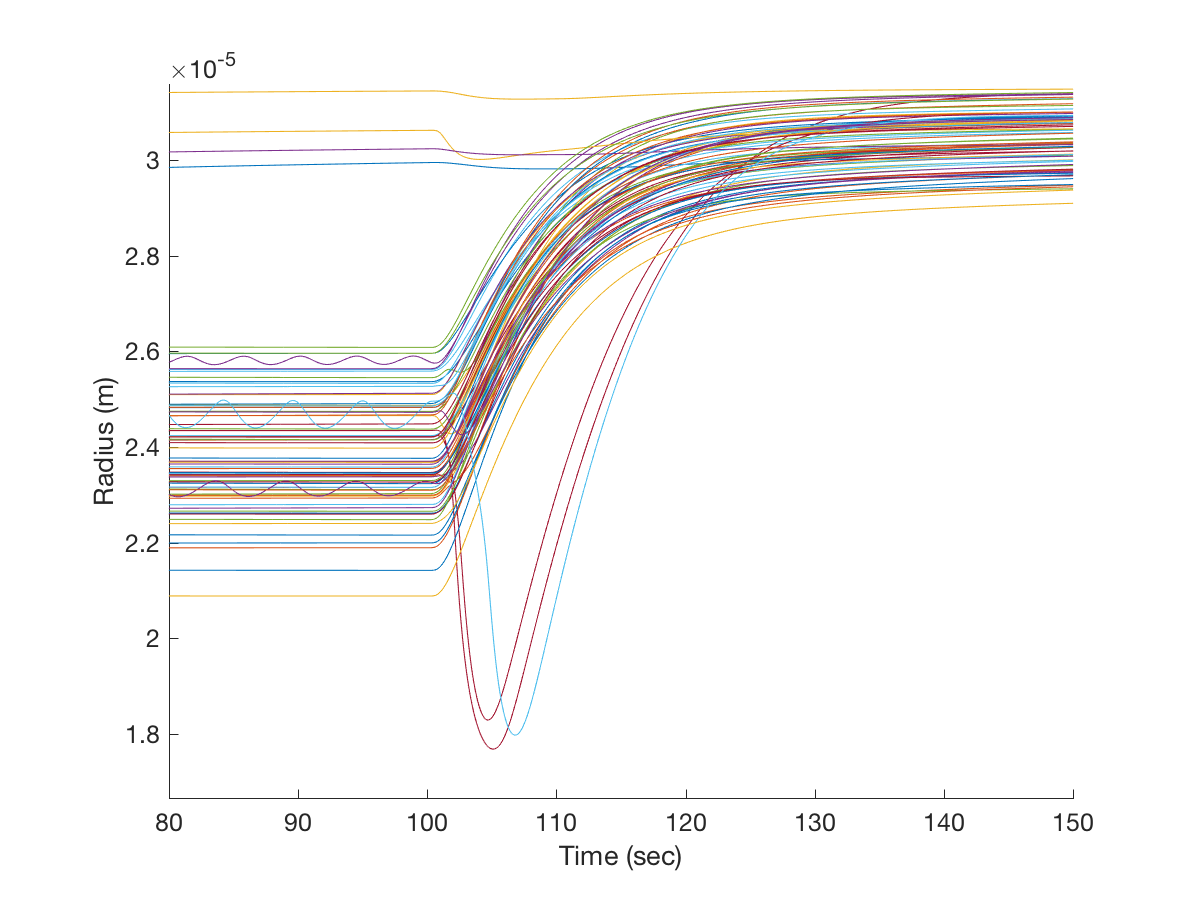
\includegraphics[width=.3 \textwidth]{Figures/Higher_Steady_State.eps}
\caption{Radii corresponding to samples (using the rectangular pulse stimulus). Left: curves an an increase in response to the stimulus; center: curves with a decrease in response to the stimulus; right: curves which settle in a different steady state.}
\label{solution_regimes}
\end{figure}

This article focuses on the typical case so we remove samples where the radius does not increase in response to the stimulus and decrease when it is removed. This processing yields 660 samples for analysis when the rectangular pulse stimulus is applied and 438 samples when the stimulus from experimental data is applied. The results presented below use these samples.

Exploration of the 660 retained samples indicate that atypical cases have higher probability when the parameter 34.9 in m2alpha is small; however, this parameter does not characterize the solution regime by itself; it is likely that the solution regime is characterized by a combination of several parameters. Further sampling and exploration is required to better understand the structure in parameter space which determine the solution regime.

\todo[inline]{I do not think we need to display BOTH the results from with the synthetic and non-synthetic stimuli. We can certainly discuss results for both, but, in the eye ball norm, the GSA results for all three QoIs are essentially identical.} 


\subsection{QoI \eqref{K_ECS_Mean} ($K_{ECS}$ Mean)}
\label{sec:qoi_K_ECS_Mean}

Figure~\ref{fig:K_ECS_Mean} displays results for the average of the ECS potassium. Across the top and bottom rows we present results for the rectangular pulse stimulus and experimental data stimulus, respectively. In the leftmost panel, predictions of the linear regression surrogate are plotted against the model values. The sensitivities $L_k$, $k=1,2,\dots,160$, are displayed in the center-left panel. Predictions of the PC surrogate are plotted against the model values in the center-right panel. The total Sobol' indices of the PC surrogate are given in the rightmost panel. Table~\ref{tab:K_ECS_Mean} reports the 5 most important parameters and their total Sobol' indices.

\begin{figure}[h]
\centering
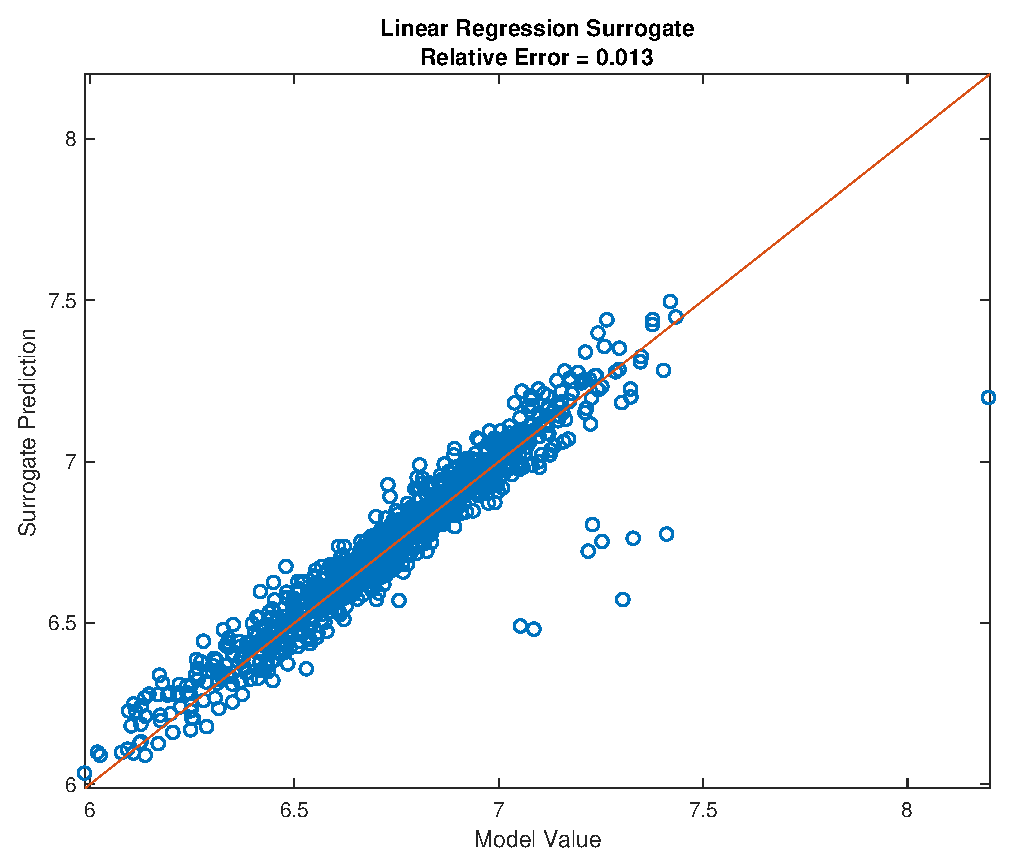
\includegraphics[width=.24 \textwidth]{Figures/K_ECS_Mean_QoI_LR_Prediction_Rectangular.eps}
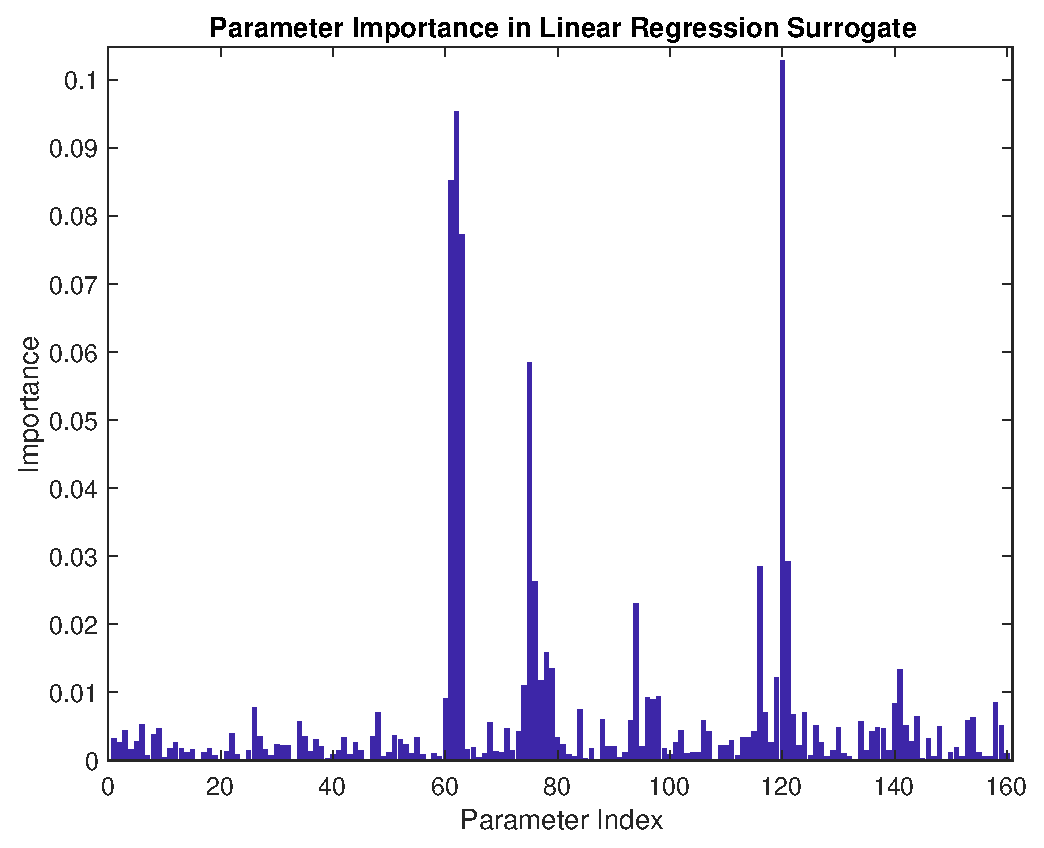
\includegraphics[width=.24 \textwidth]{Figures/K_ECS_Mean_QoI_LR_VI_Rectangular.eps}
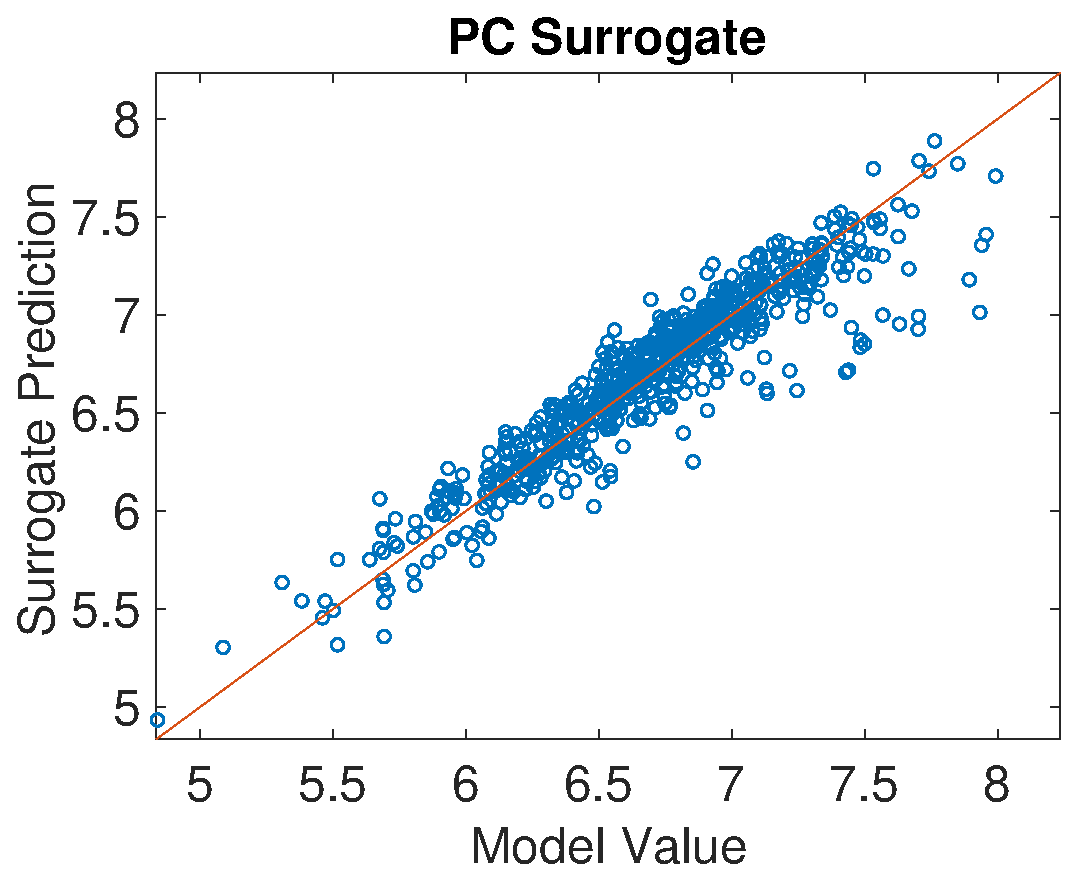
\includegraphics[width=.24 \textwidth]{Figures/K_ECS_Mean_QoI_PCE_Prediction_Rectangular.eps}
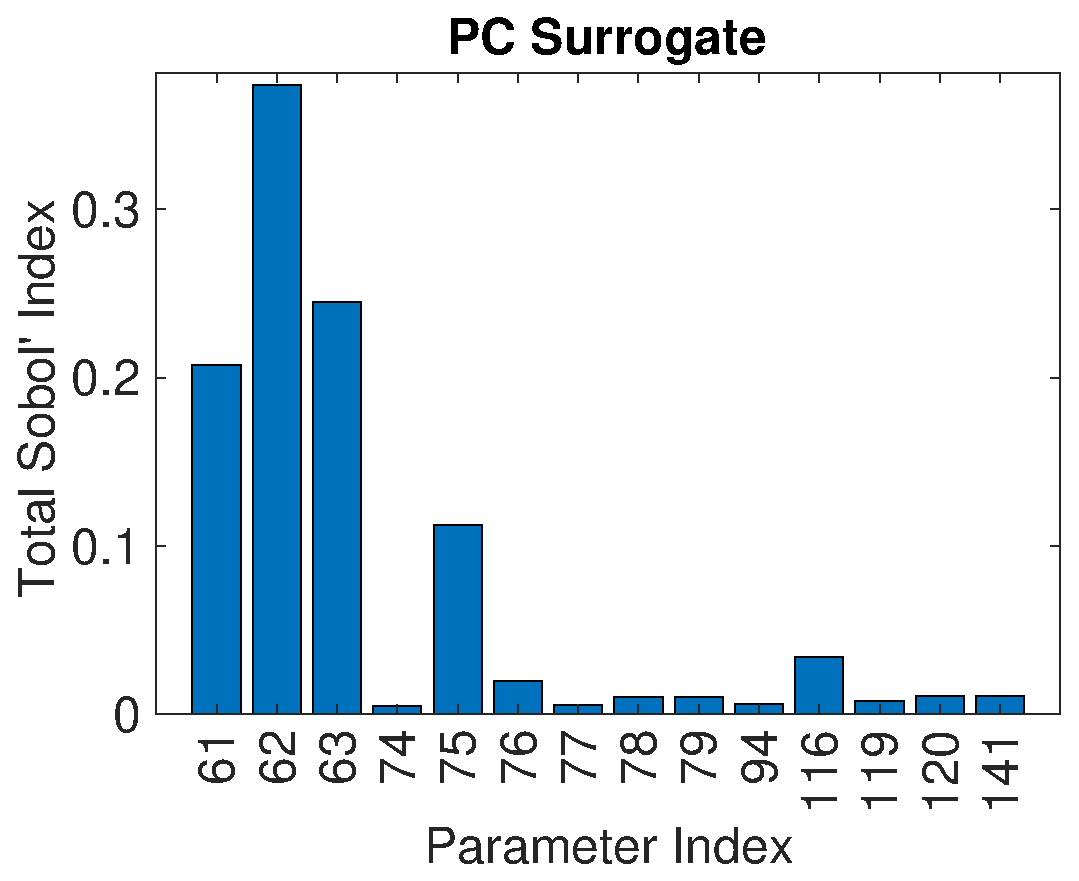
\includegraphics[width=.24 \textwidth]{Figures/K_ECS_Mean_QoI_PCE_SI_Rectangular.eps}\\
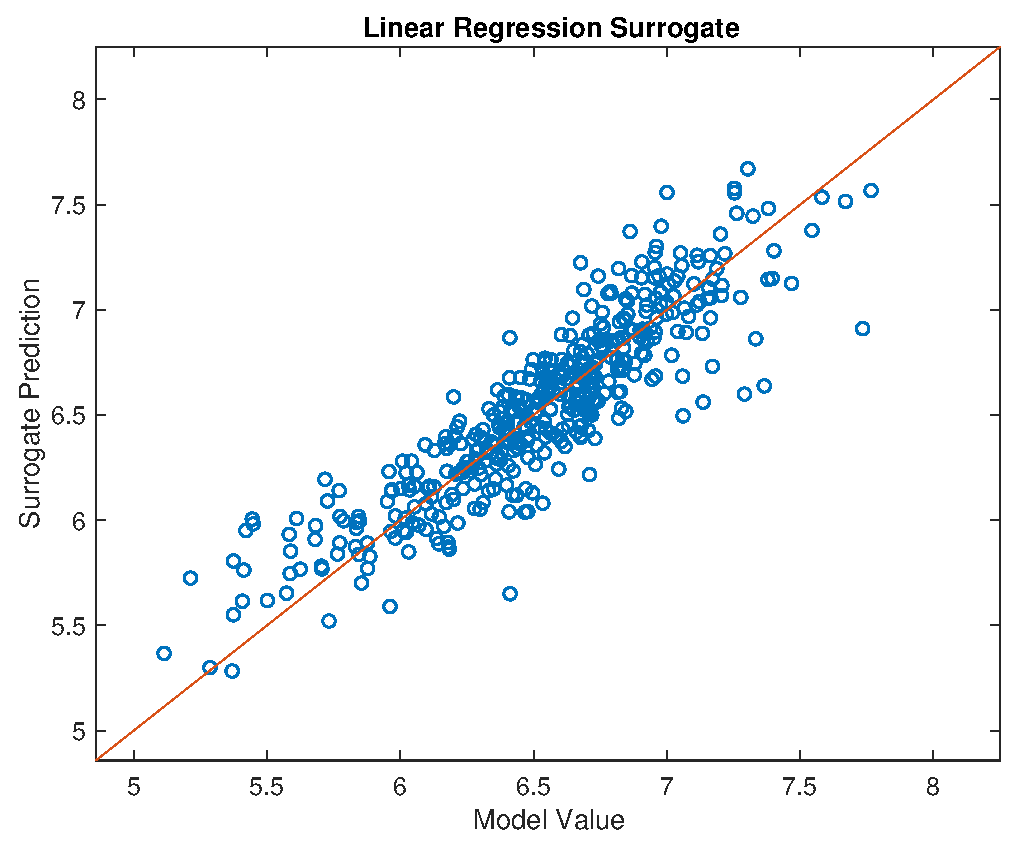
\includegraphics[width=.24 \textwidth]{Figures/K_ECS_Mean_QoI_LR_Prediction_Experimental.eps}
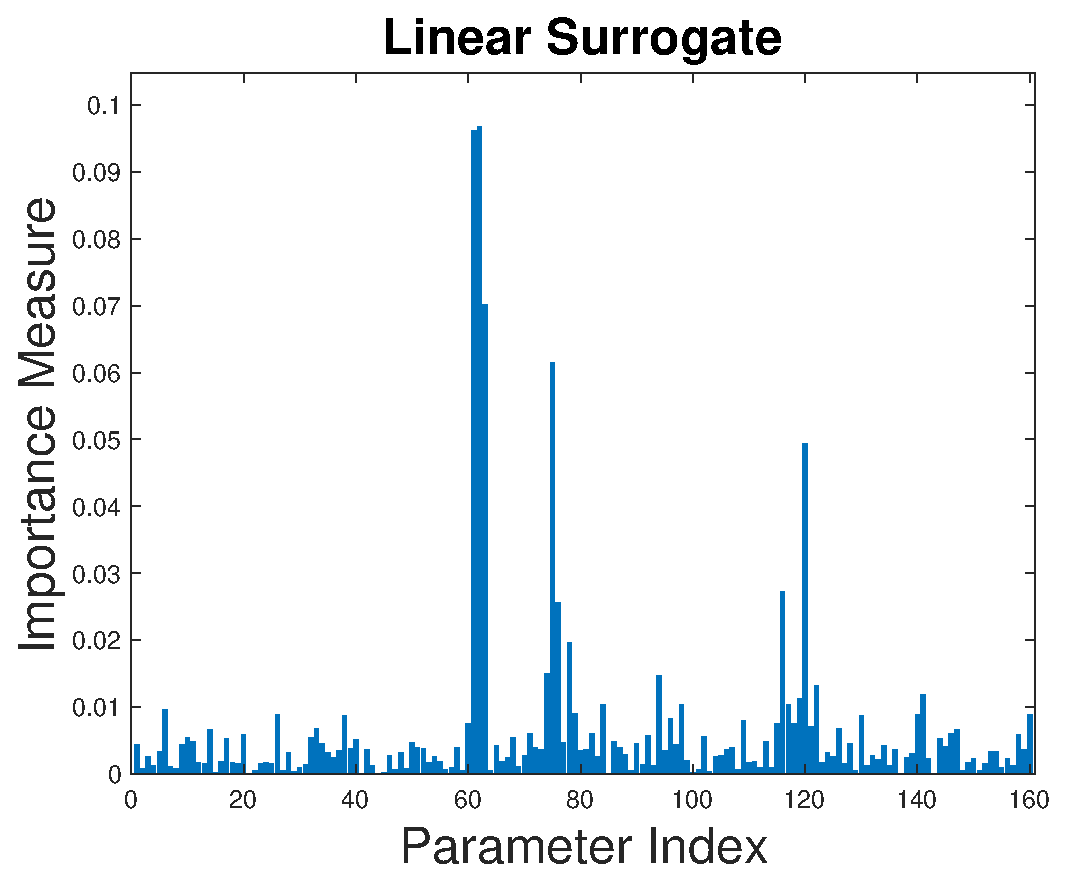
\includegraphics[width=.24 \textwidth]{Figures/K_ECS_Mean_QoI_LR_VI_Experimental.eps}
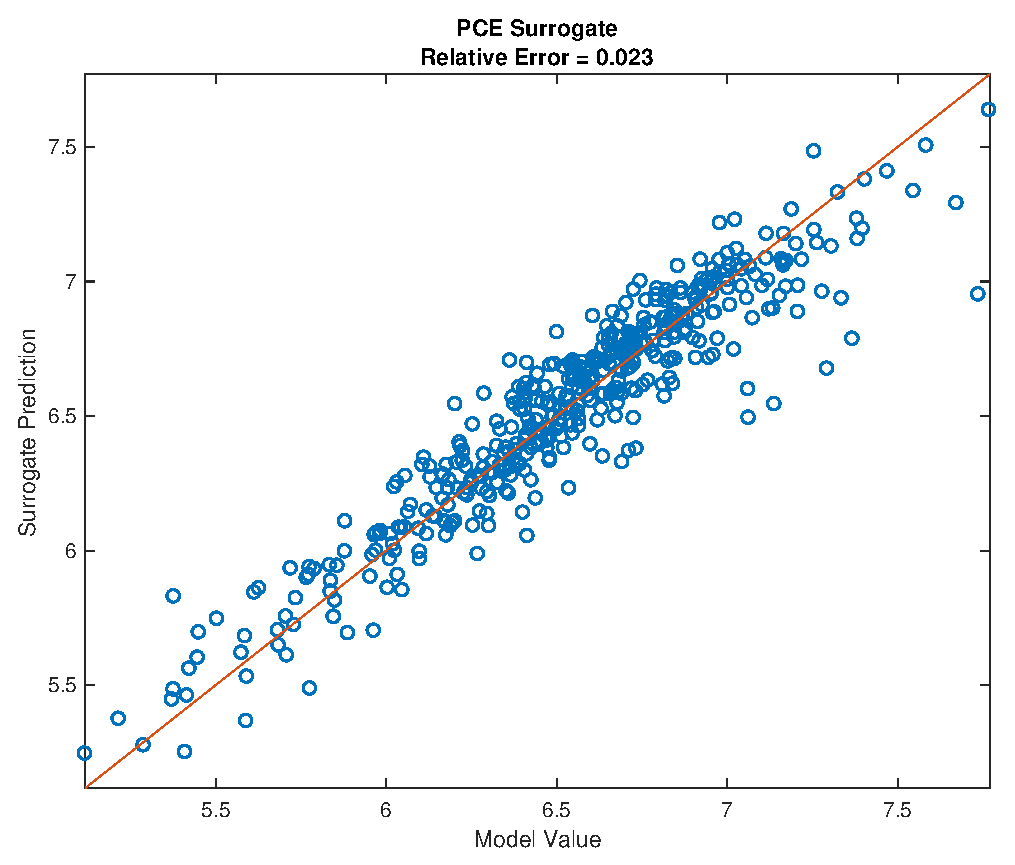
\includegraphics[width=.24 \textwidth]{Figures/K_ECS_Mean_QoI_PCE_Prediction_Experimental.eps}
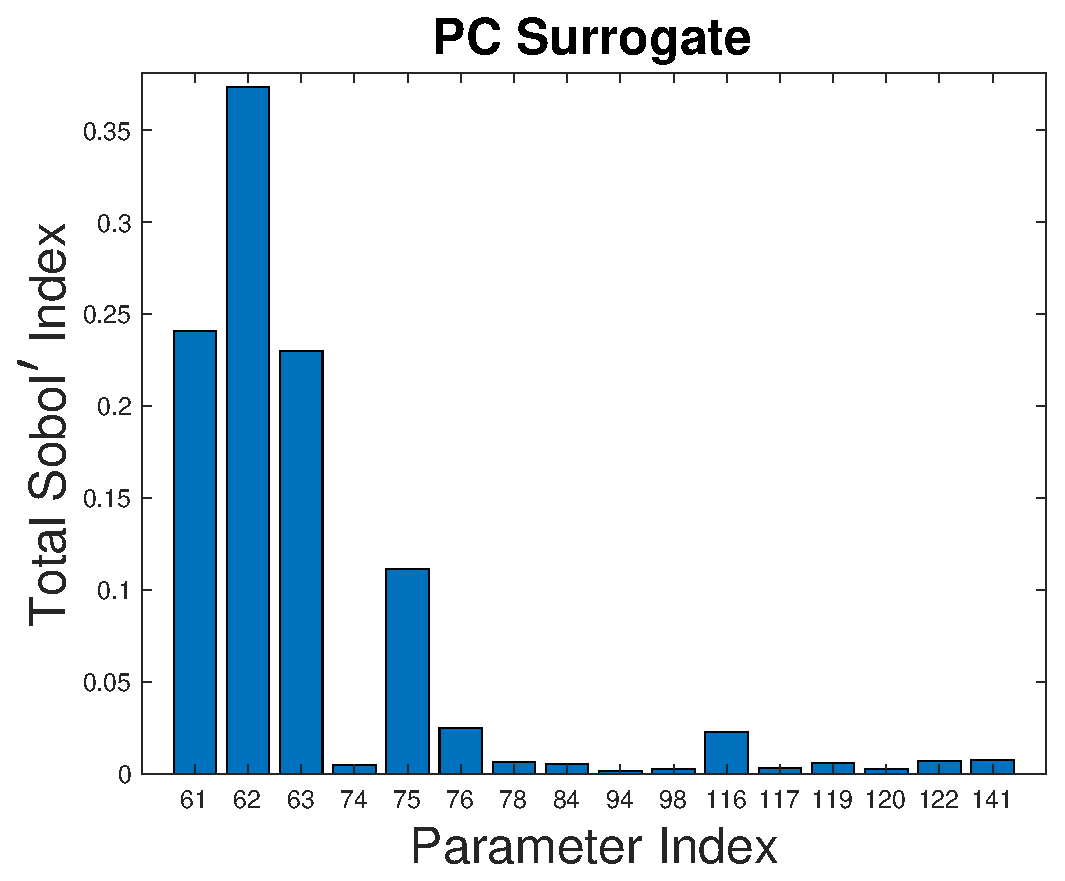
\includegraphics[width=.24 \textwidth]{Figures/K_ECS_Mean_QoI_PCE_SI_Experimental.eps}
\caption{Results for ECS potassium QoI. Top row: results with a rectangular pulse stimulus; bottom row: results with experimental data stimulus. From left to right, linear regression predictions, linear regression variable importance, PCE predictions, total Sobol' indices for PCE.}
\label{fig:K_ECS_Mean}
\end{figure}

    0.3715
    0.2488
    0.2092
    0.1236
    0.0371

\begin{table}[h]
\centering
\begin{tabular}{cccc}
Index & Identification & Total Sobol' Index (RP) & Total Sobol' Index (ES)\\
62 & 0.143 in m4alpha and m4 beta &  0.3715 & 0.3682\\
63 & 5.67 in m4alpha and m4 beta &  0.2488 & 0.2313\\
61 & gKleak\_d in Neuron & 0.2092 & 0.2483\\
75 & 34.9 in m6alpha & 0.1236 & 0.1068\\
116 & dhod in Neuron &   0.0371 & 0.0256\\
\end{tabular}
\caption{Most influential parameters for the ECS potassium QoI.}
\label{tab:K_ECS_Mean}
\end{table}

The results are similar for both the rectangular pulse and experimental data stimulus. In both cases, the QoI is approximated with reasonable accuracy by a linear model and with higher accuracy by the PC model. The most important parameters are shared in both cases. Notice that parameter 120 appears to be important in the linear model but unimportant in the PC model. This is because it is strongly correlated with parameter 121, see Figure~\ref{steady_states} and the discussion in Subsection~\ref{sec:param_sampling}, and as a result the coefficient in linear regression may be very large because its effect is offset by the effect of parameter 121. To decorrelate inputs, the PC surrogate is build with only parameter 120 instead of both 120 and 121. It subsequently has minimal importance.

\subsection{QoI \eqref{vol_flow} (volumetric flow rate)}

Figure~\ref{fig:qoi_vol_flow} displays results for the volumetric flow rate in the cerebral tissue. In the same manner as Figure~\ref{fig:K_ECS_Mean}, the linear and PC surrogate predictions and sensitivities are plotted for both the rectangular pulse and experimental data stimulus. Table~\ref{tab:qoi_vol_flow} reports the 5 most important parameters and their total Sobol' indices.

\begin{figure}[h]
\centering
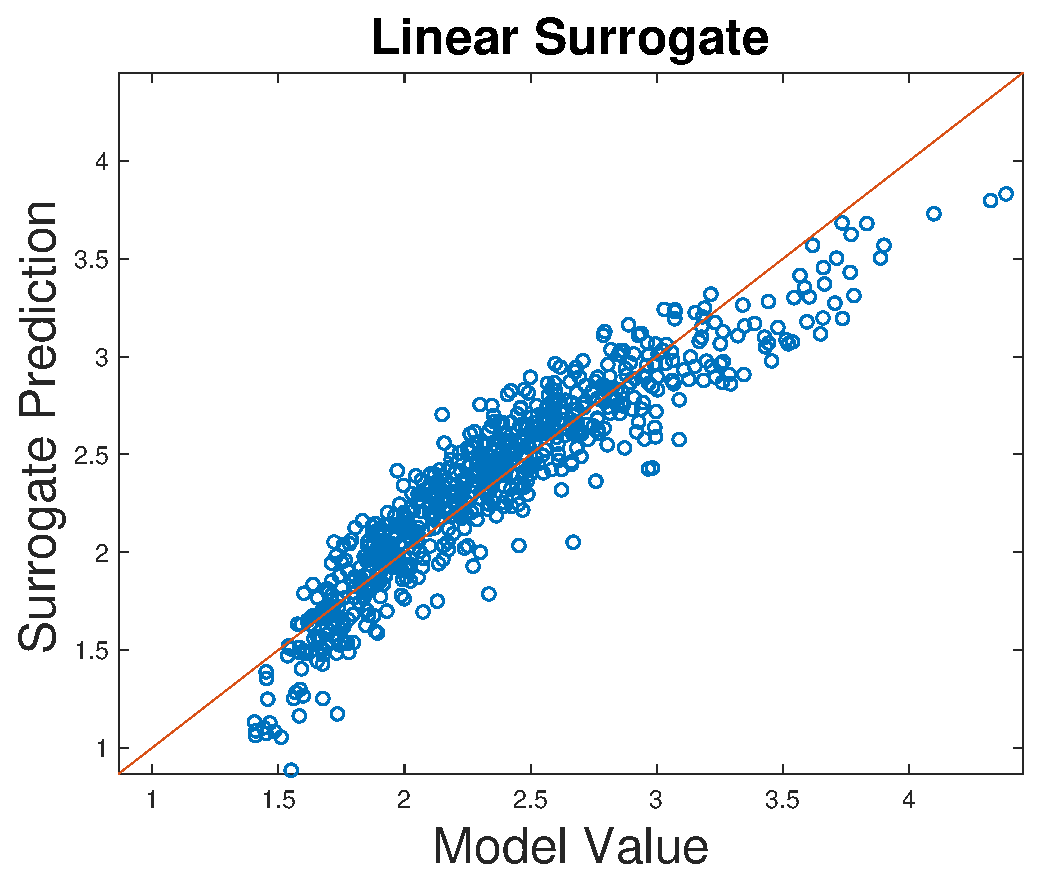
\includegraphics[width=.24 \textwidth]{Figures/Vol_Flow_QoI_LR_Prediction_Rectangular.eps}
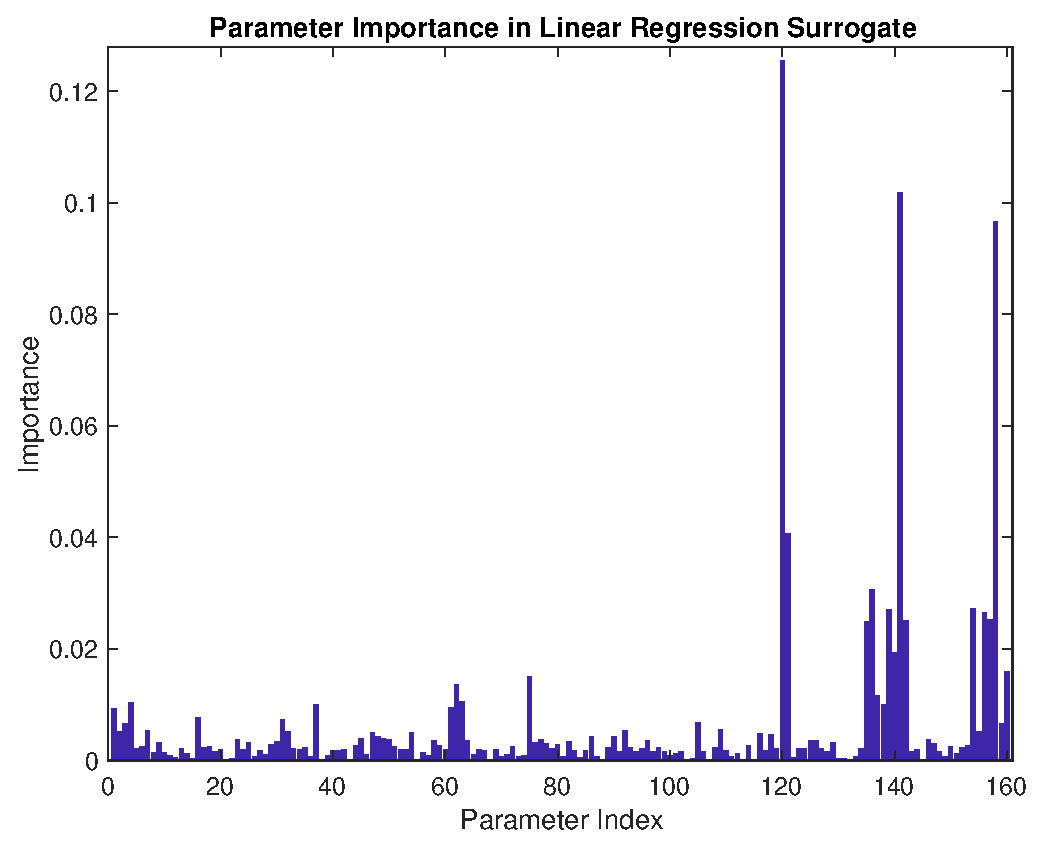
\includegraphics[width=.24 \textwidth]{Figures/Vol_Flow_QoI_LR_VI_Rectangular.eps}
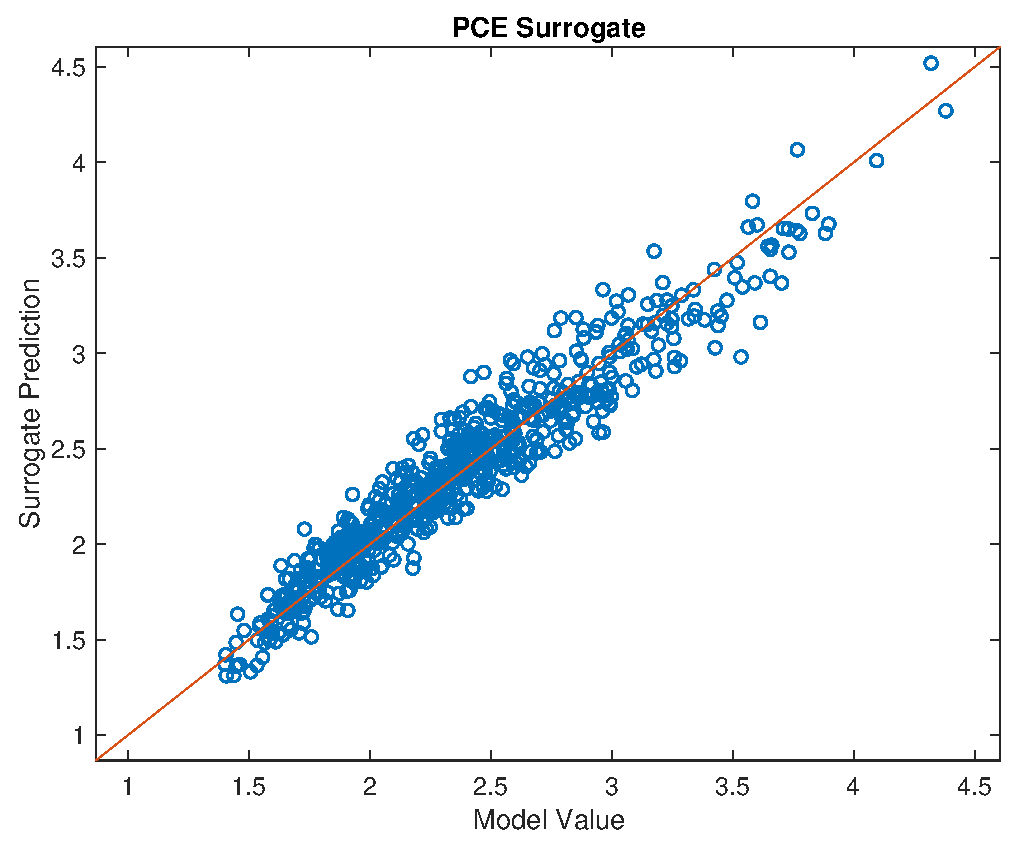
\includegraphics[width=.24 \textwidth]{Figures/Vol_Flow_QoI_PCE_Prediction_Rectangular.eps}
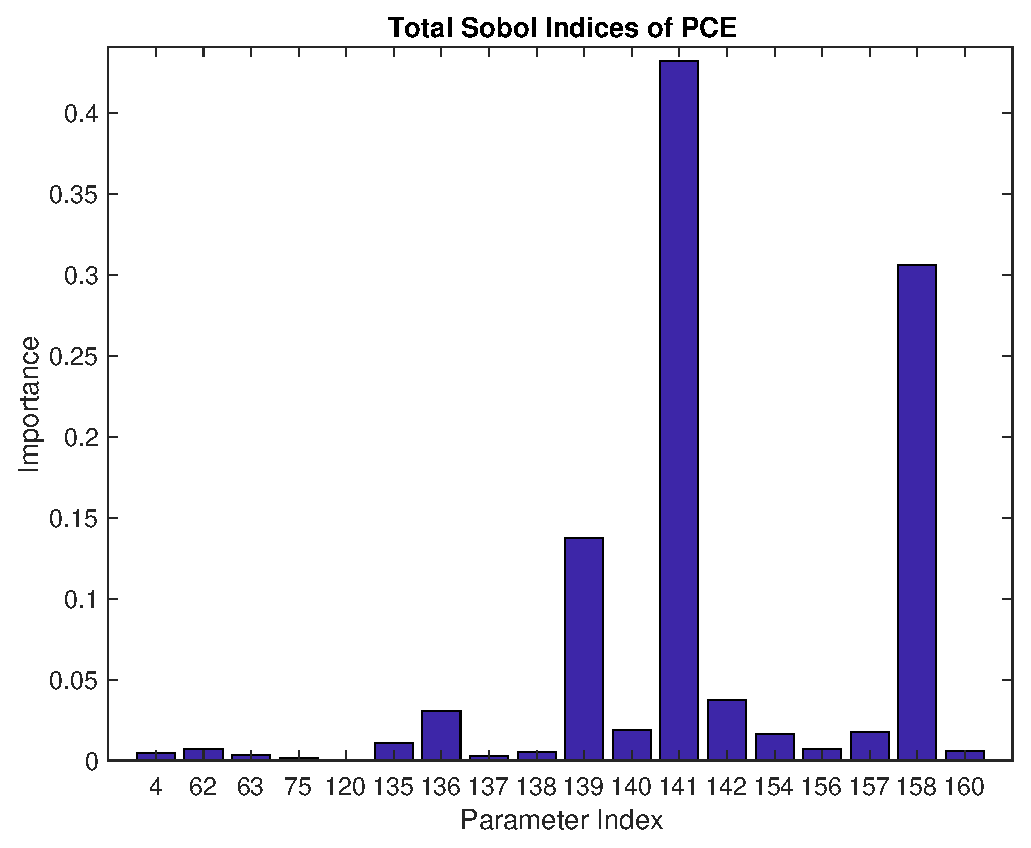
\includegraphics[width=.24 \textwidth]{Figures/Vol_Flow_QoI_PCE_SI_Rectangular.eps}\\
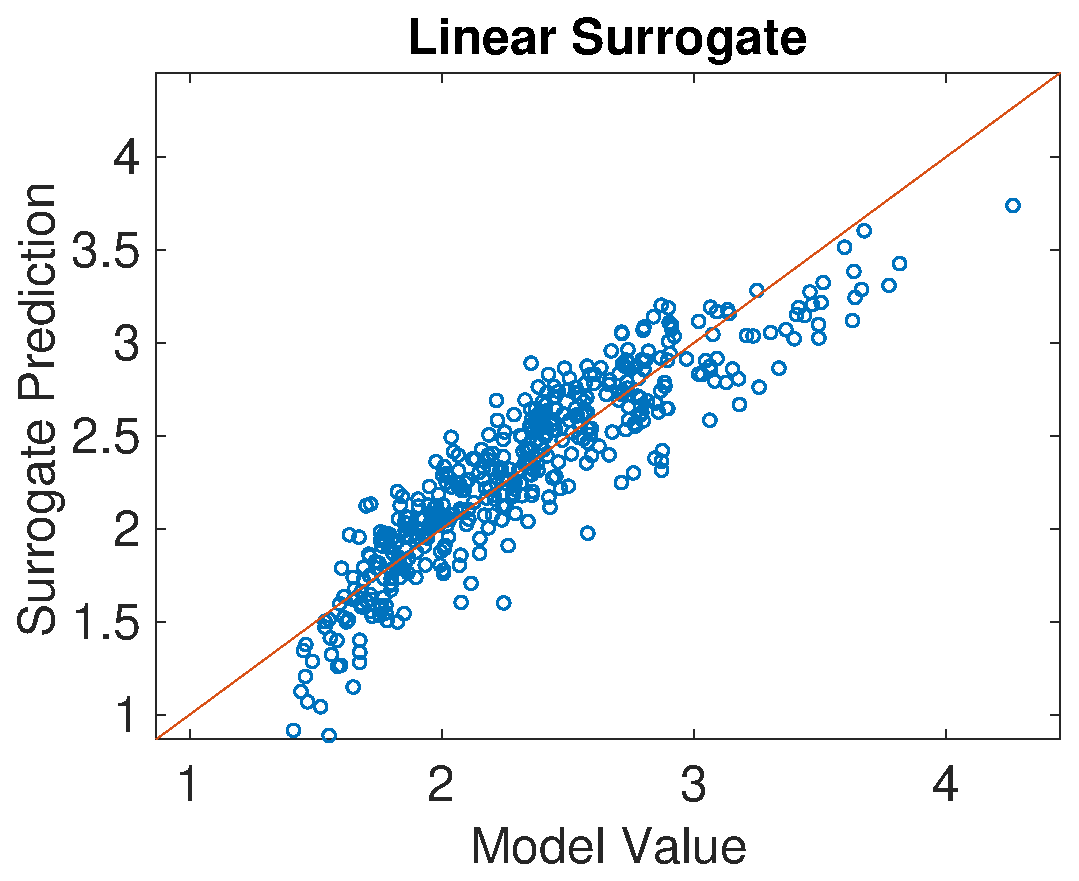
\includegraphics[width=.24 \textwidth]{Figures/Vol_Flow_QoI_LR_Prediction_Experimental.eps}
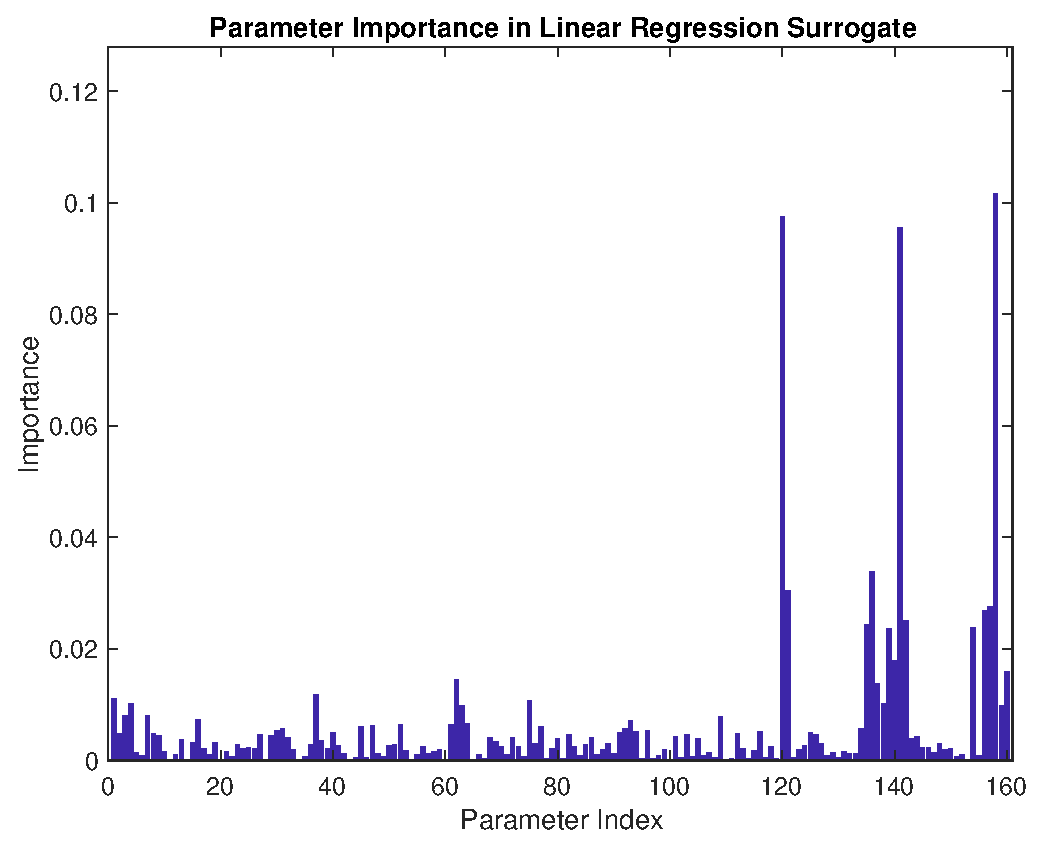
\includegraphics[width=.24 \textwidth]{Figures/Vol_Flow_QoI_LR_VI_Experimental.eps}
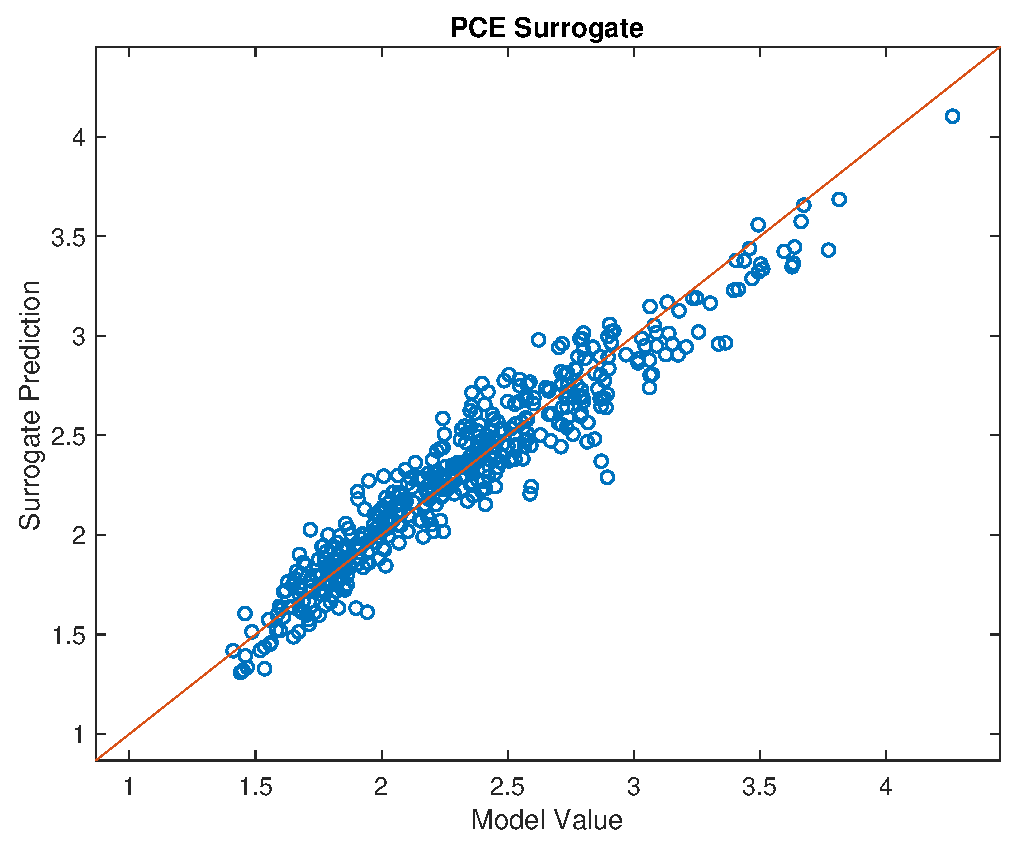
\includegraphics[width=.24 \textwidth]{Figures/Vol_Flow_QoI_PCE_Prediction_Experimental.eps}
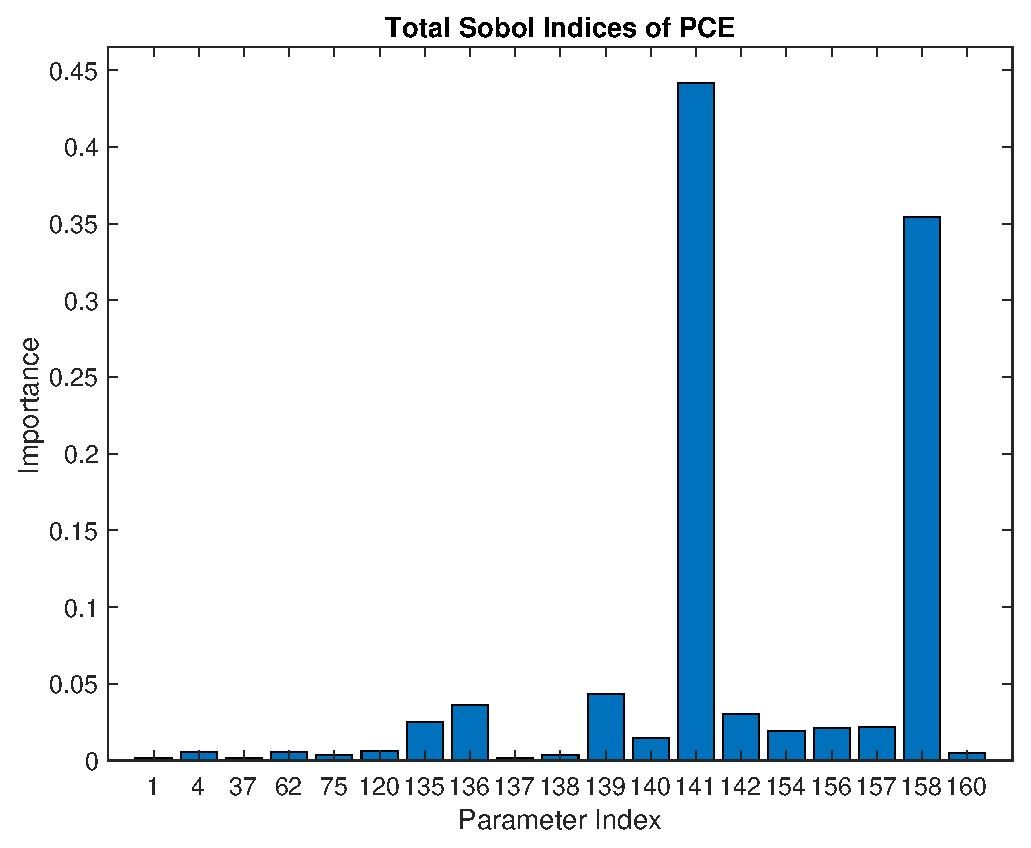
\includegraphics[width=.24 \textwidth]{Figures/Vol_Flow_QoI_PCE_SI_Experimental.eps}
\caption{Results for the volumetric flow rate in the cerebral tissue QoI. Top row: results with a rectangular pulse stimulus; bottom row: results with experimental data stimulus. From left to right, linear regression predictions, linear regression variable importance, PCE predictions, total Sobol' indices for PCE.}
\label{fig:qoi_vol_flow}
\end{figure}

We again observe reasonably accurate fits by a linear surrogate and improved accuracy by a PC surrogate. The surrogate predictions and important parameters for the rectangular pulse and experimental stimulus closely agree. The influential parameters for the volumetric flow rate in the cerebral tissue are different than those found to be influential for the ECS potassium. This is an unsurprising result. As in Subsection~\ref{sec:qoi_K_ECS_Mean}, parameter 120 appears important in the linear surrogate but unimportant in the PC surrogate.

\begin{table}[h]
\centering
\begin{tabular}{cccc}
Index & Identification & Total Sobol' Index (RP) & Total Sobol' Index (ES)\\
141 &  z\_4 in SMCEC & 0.4320 & 0.3871\\
158 & n\_cross in WallMechanics & 0.3059 & 0.2948\\ 
 139 & z\_2 in SMCEC & 0.1371 & 0.1265\\
 142 & z\_5 in SMCEC & 0.0376 & 0.0350\\
  136 & G\_K\_i in SMCEC & 0.0303 & 0.0300\\
\end{tabular}
\caption{Most influential parameters for the volumetric flow rate in the cerebral tissue QoI.}
\label{tab:qoi_vol_flow}
\end{table}

\subsection{QoI \eqref{AM_AMp_Min} ($AM+AM_p$ Min)}

Figure~\ref{fig:qoi_AM_AMp_Min} displays results for the minimum of the combined concentration of the actin myosin complex. As in the previous subsections, the linear and PC surrogate predictions and sensitivities are plotted for both the rectangular pulse and experimental data stimulus. Table~\ref{tab:qoi_AM_AMp_Min} reports the 5 most important parameters (ranked by the total Sobol' indices for the rectangular pulse stimulus) and their total Sobol' indices.

\begin{figure}[h]
\centering
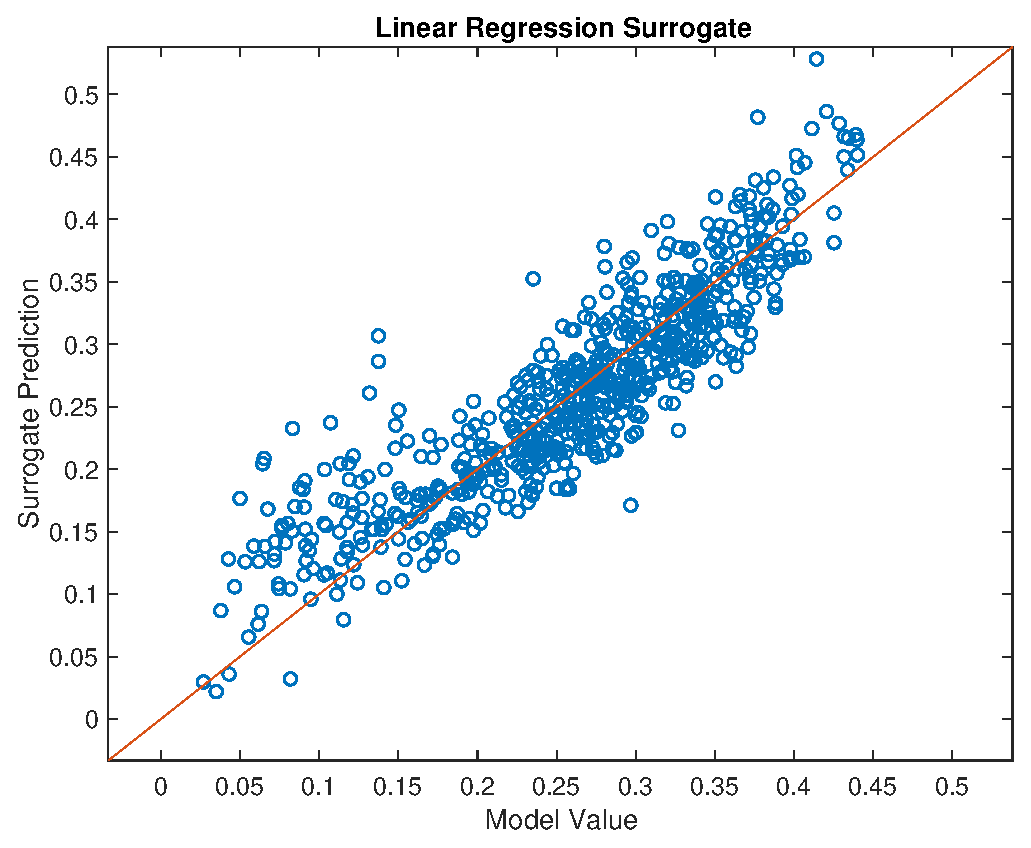
\includegraphics[width=.24 \textwidth]{Figures/AM_AMp_Min_QoI_LR_Prediction_Rectangular.eps}
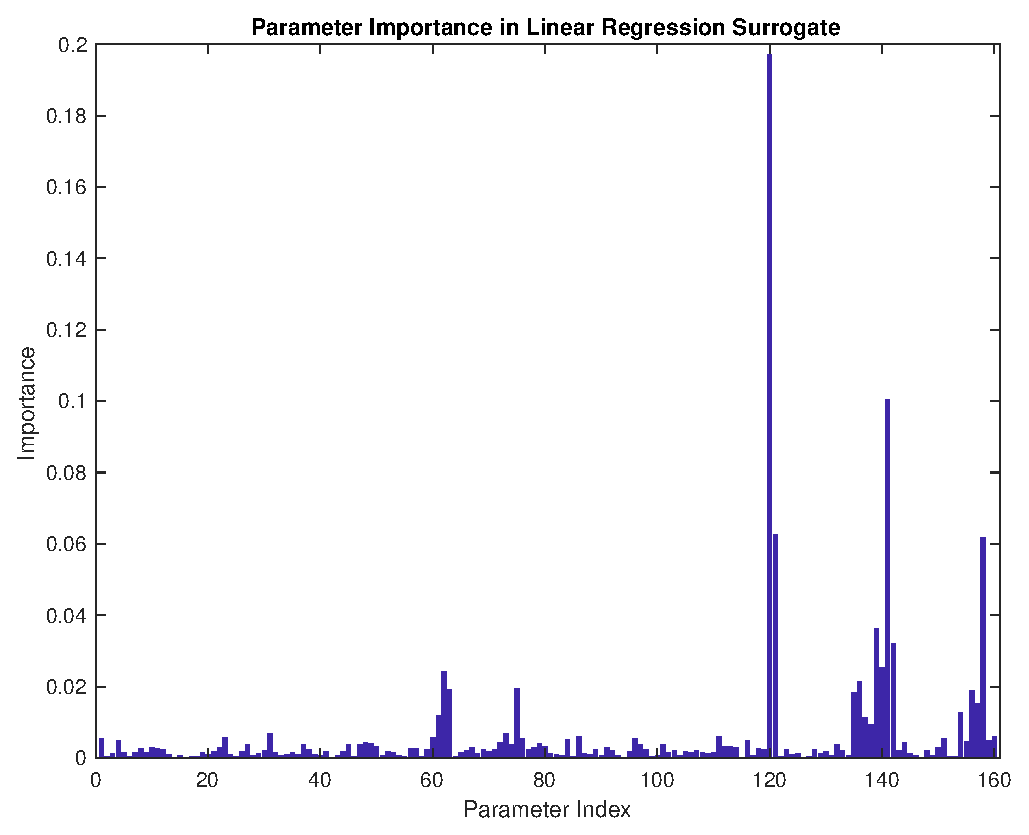
\includegraphics[width=.24 \textwidth]{Figures/AM_AMp_Min_QoI_LR_VI_Rectangular.eps}
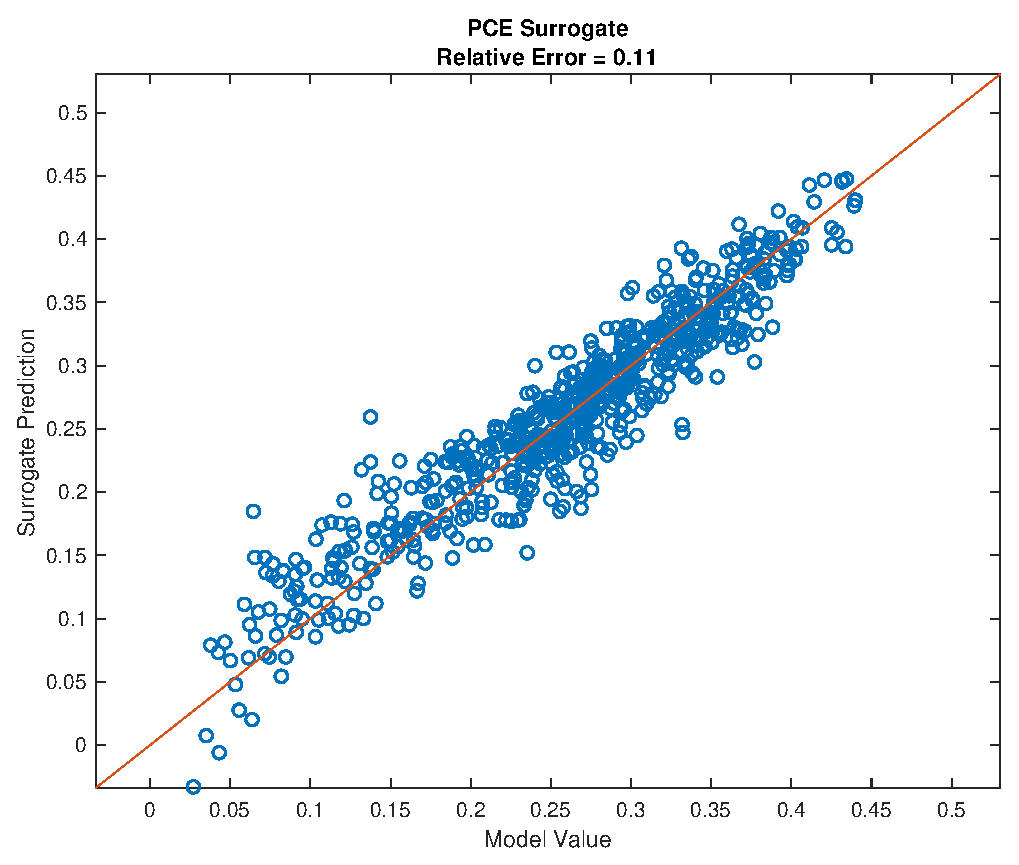
\includegraphics[width=.24 \textwidth]{Figures/AM_AMp_Min_QoI_PCE_Prediction_Rectangular.eps}
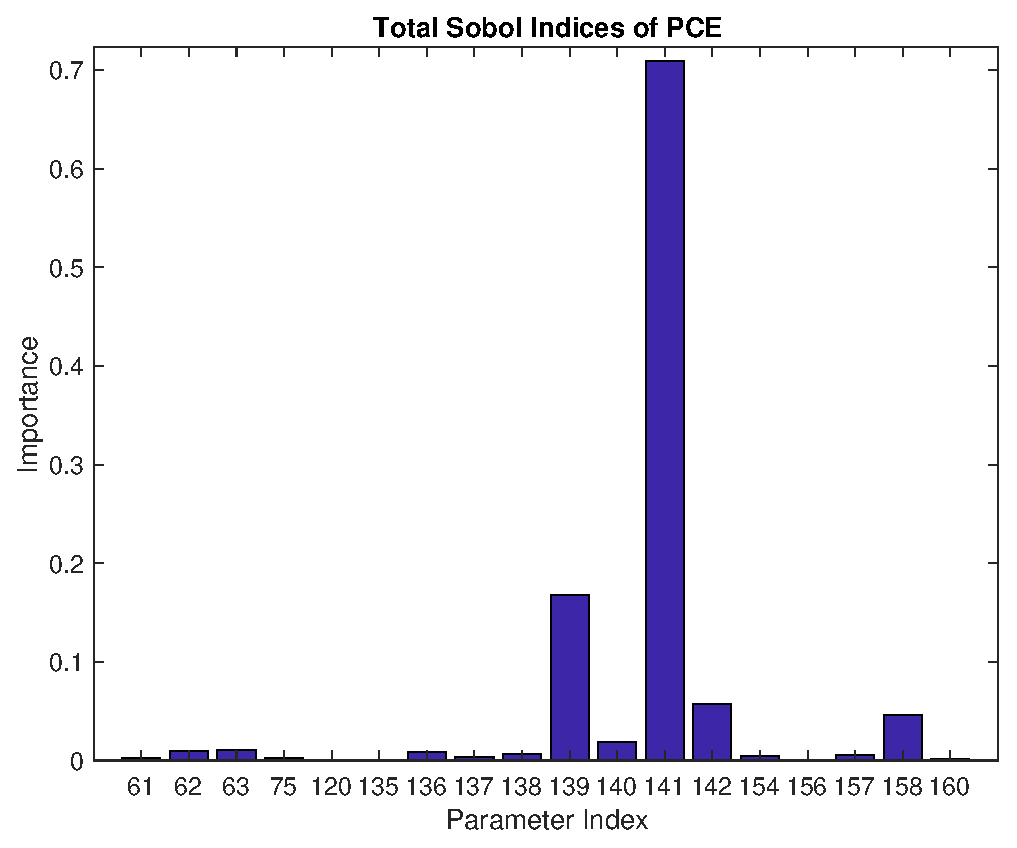
\includegraphics[width=.24 \textwidth]{Figures/AM_AMp_Min_QoI_PCE_SI_Rectangular.eps}\\
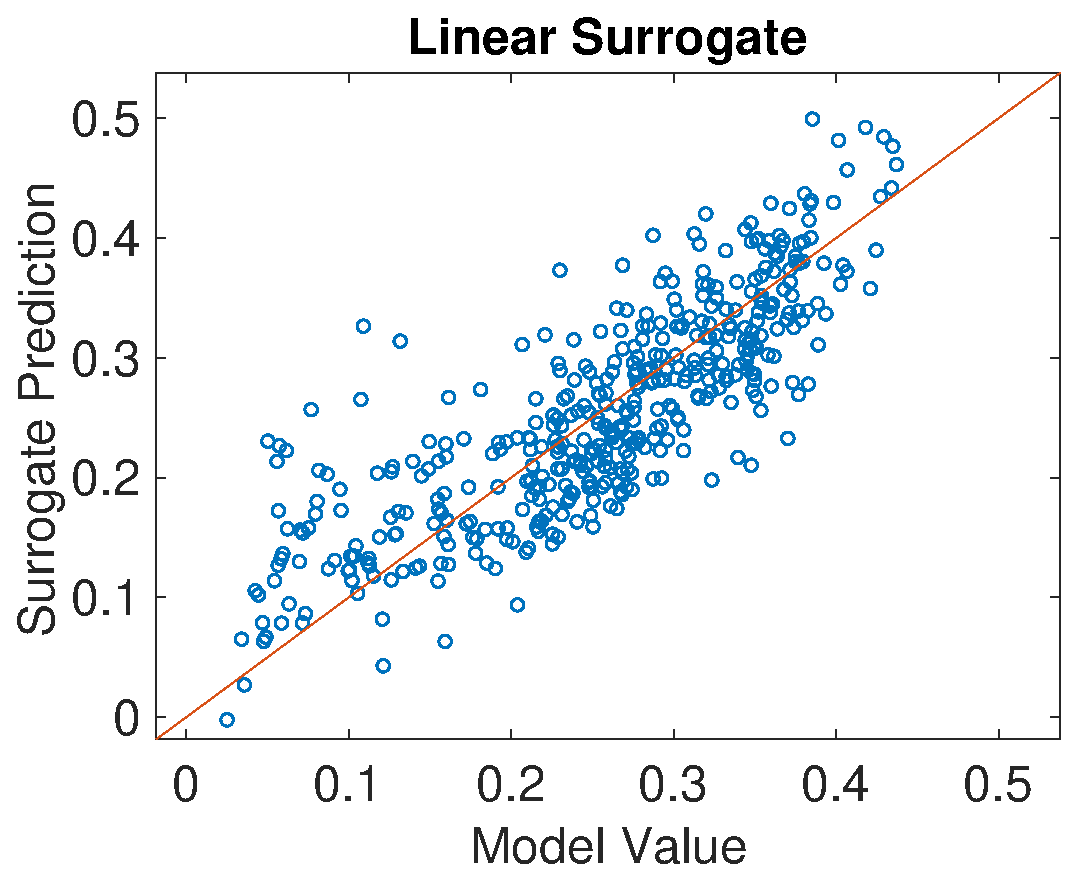
\includegraphics[width=.24 \textwidth]{Figures/AM_AMp_Min_QoI_LR_Prediction_Experimental.eps}
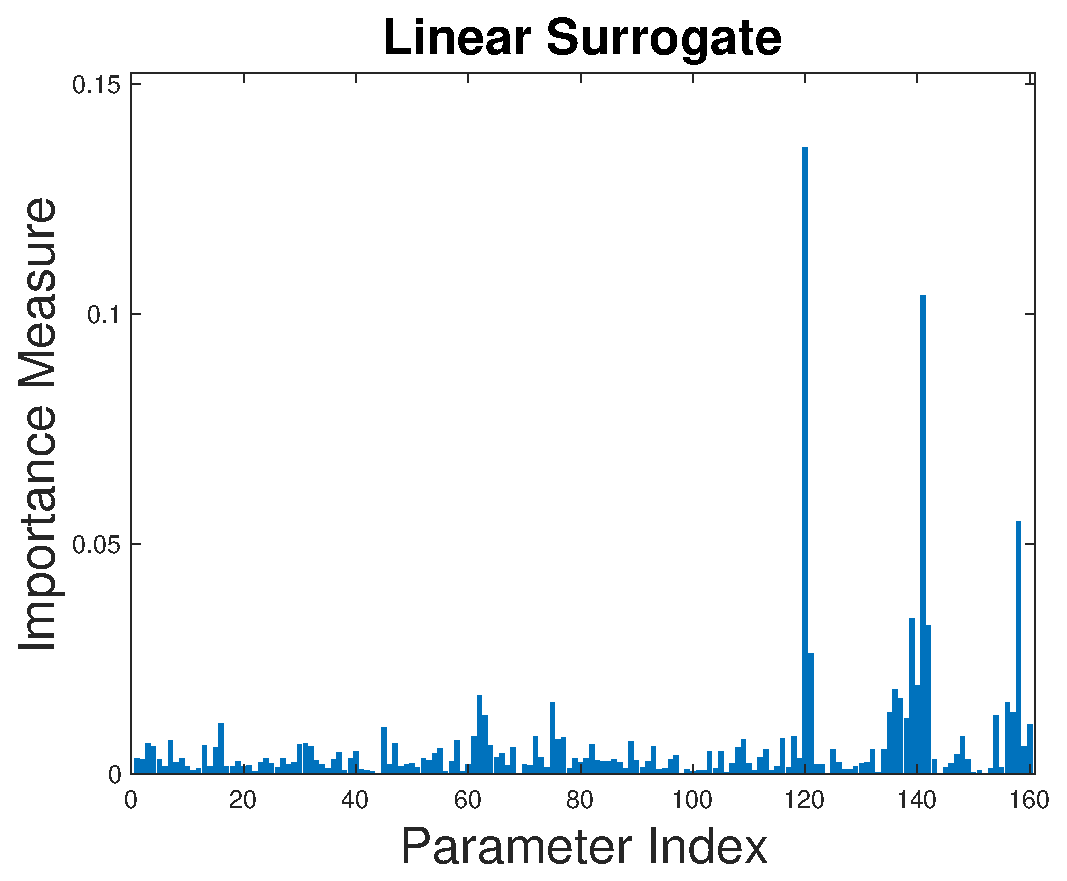
\includegraphics[width=.24 \textwidth]{Figures/AM_AMp_Min_QoI_LR_VI_Experimental.eps}
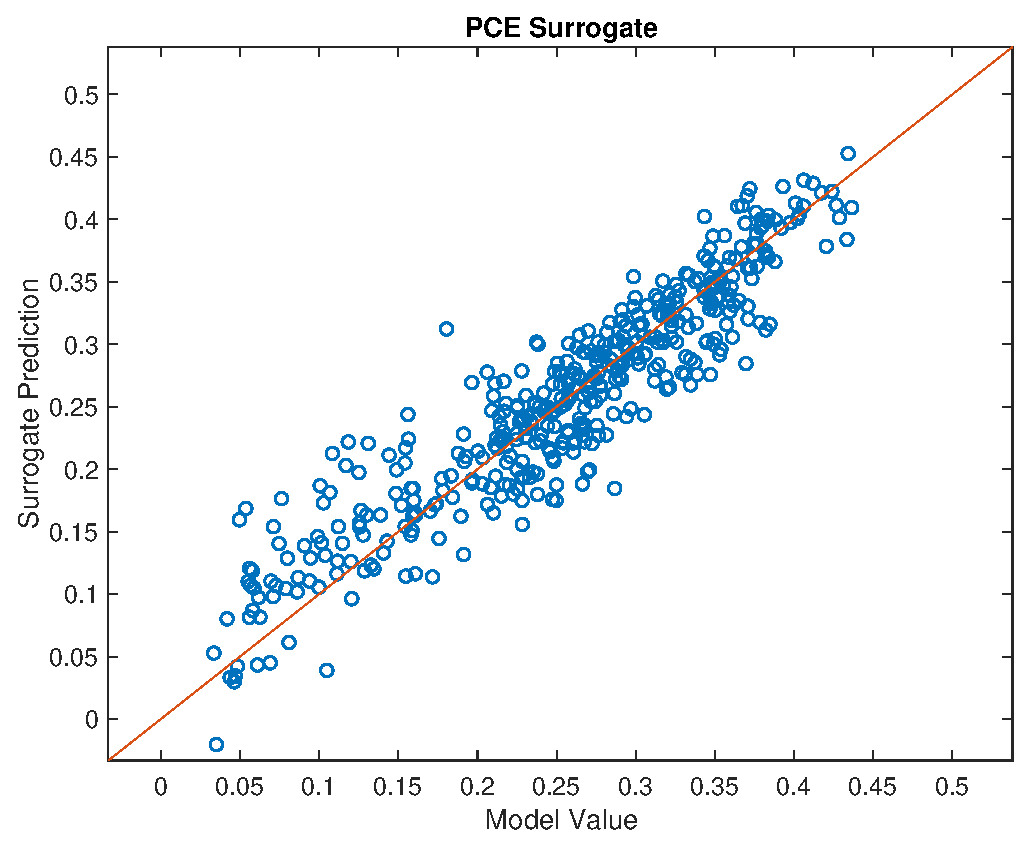
\includegraphics[width=.24 \textwidth]{Figures/AM_AMp_Min_QoI_PCE_Prediction_Experimental.eps}
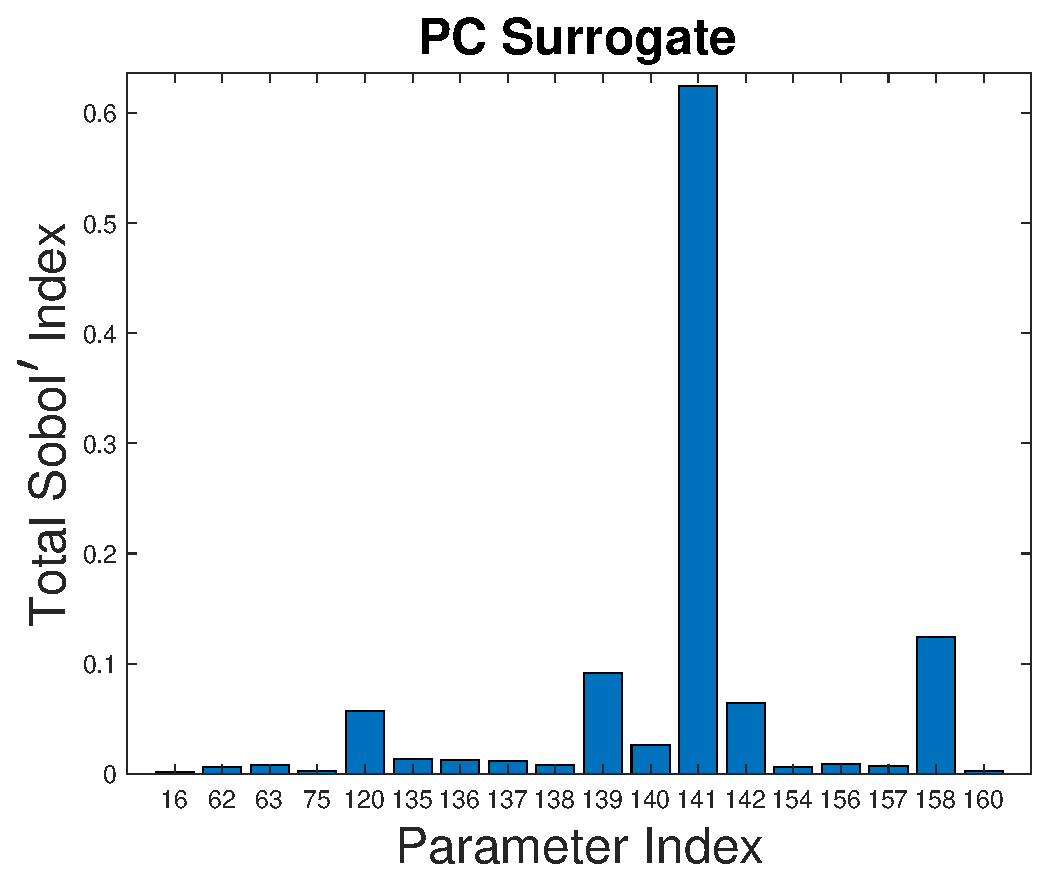
\includegraphics[width=.24 \textwidth]{Figures/AM_AMp_Min_QoI_PCE_SI_Experimental.eps}
\caption{Results for the minimum of the combined concentration of the actin myosin complex QoI. Top row: results with a rectangular pulse stimulus; bottom row: results with experimental data stimulus. From left to right, linear regression predictions, linear regression variable importance, PCE predictions, total Sobol' indices for PCE.}
\label{fig:qoi_AM_AMp_Min}
\end{figure}

The linear surrogate does not perform as well for this QoI; however, the PC surrogate is far more accurate; this highlights the nonlinearity of the QoI. The subset of parameters used in the PC surrogate differs for the rectangular pulse and experimental stimulus cases, but the most important parameters, as measured by the total Sobol' indices, agree. The most influential parameters for the minimum of the combined concentration of the actin myosin complex coincide with those for the volumetric flow rate in the cerebral tissue, an unsurprising result since both QoI are related to the wall mechanics. Parameter 120 appears important in the linear surrogate but unimportant in the PC surrogate.

\begin{table}[h]
\centering
\begin{tabular}{cccc}
Index & Identification & Total Sobol' Index (RP) & Total Sobol' Index (ES)\\
141 & z\_4 in SMCEC & 0.7091 & 0.6567\\
139 &  z\_2 in SMCEC & 0.1682 & 0.1641\\
142 & z\_5 in SMCEC & 0.0570 & 0.0332\\
158 & n\_cross in WallMechanics & 0.0462 & 0.0651\\
140 & z\_3 in SMCEC & 0.0188 &0.0130\\
\end{tabular}
\caption{Most influential parameters for the combined concentration of the actin myosin complex QoI.}
\label{tab:qoi_AM_AMp_Min}
\end{table}

\section{Extra figures we probably won't include}
\subsection{$AM_p$ Time Lag}

\begin{figure}[h]
\centering
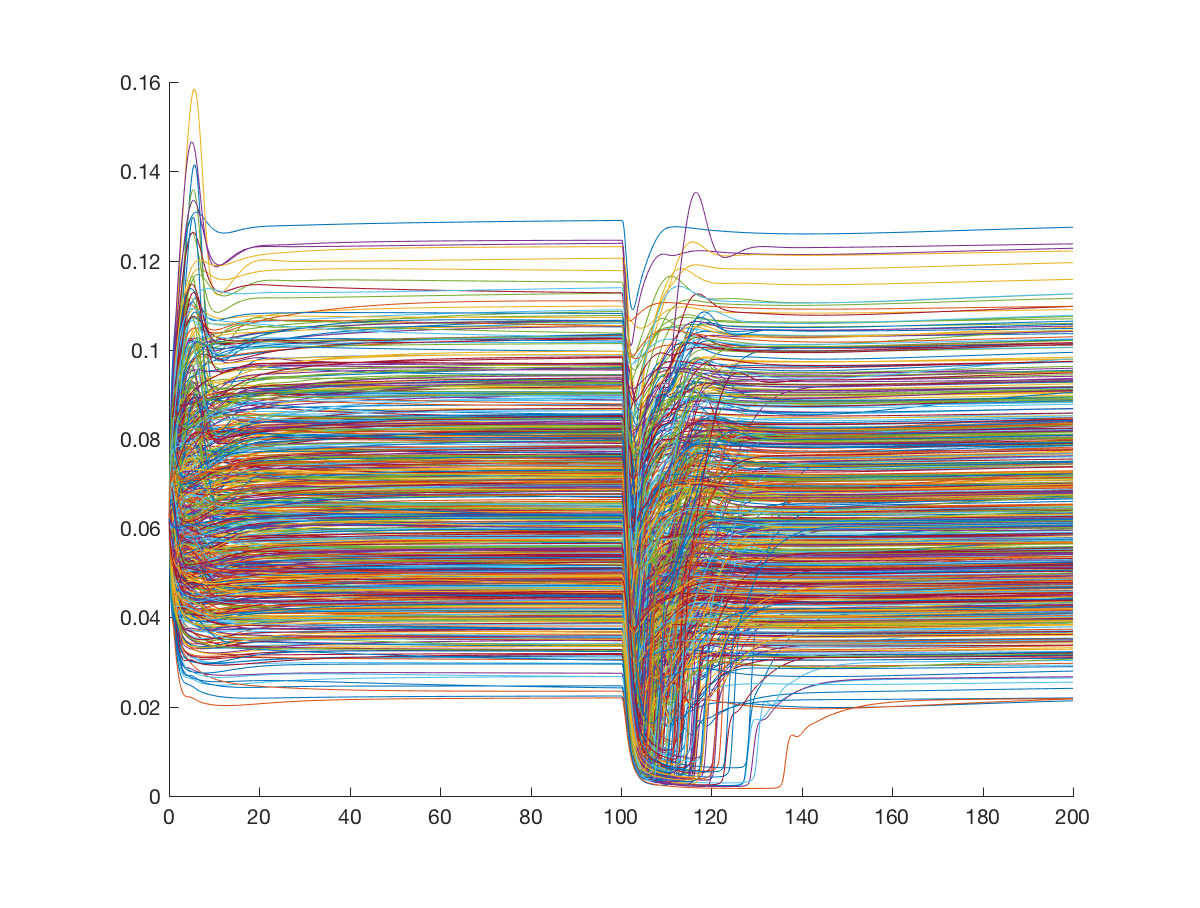
\includegraphics[width=.49 \textwidth]{Figures/AMp_Curves.eps}
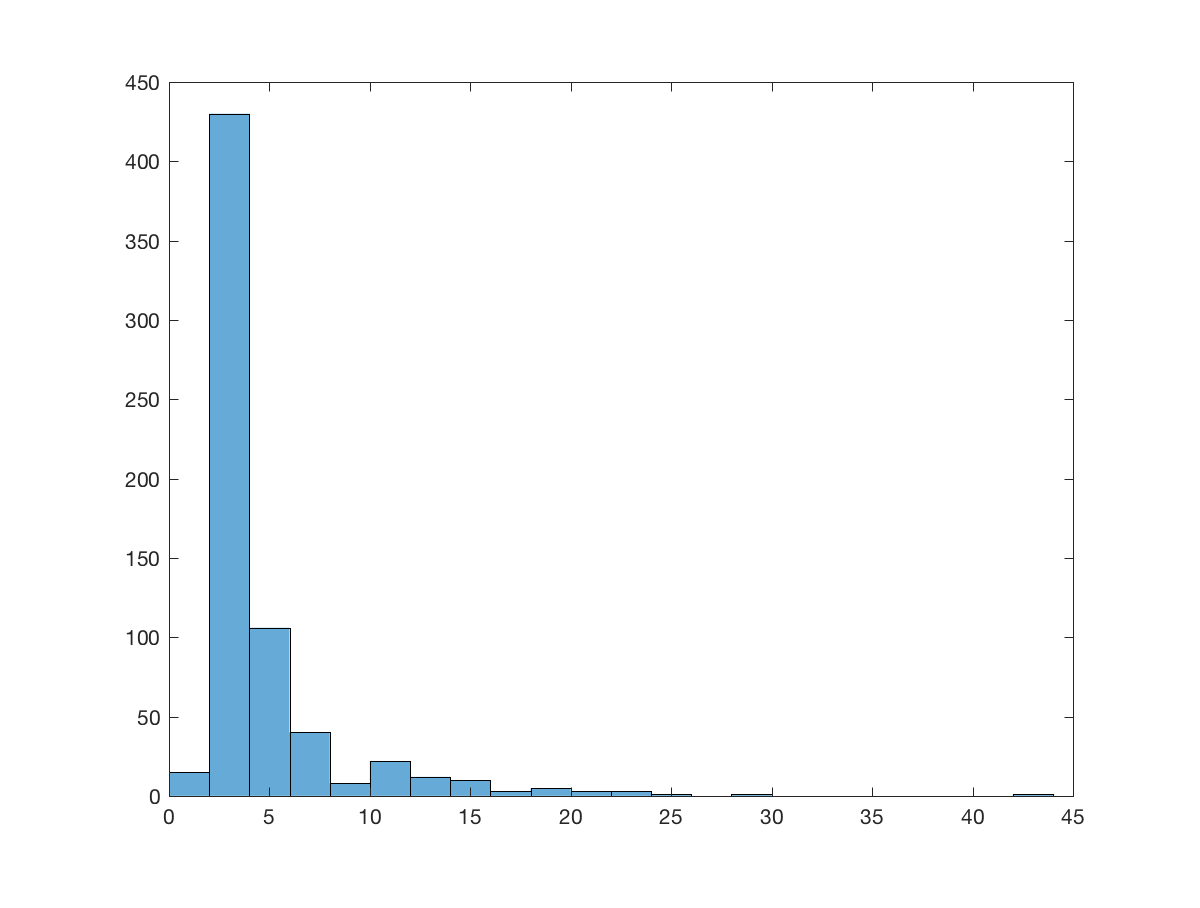
\includegraphics[width=.49 \textwidth]{Figures/AMp_Time_Lag_Histogram.eps}
\caption{$AM_p$ curves on the left and a histogram of the time lags on the right.}
\end{figure}

\subsection{Radius Time Lag}

\begin{figure}[h]
\centering
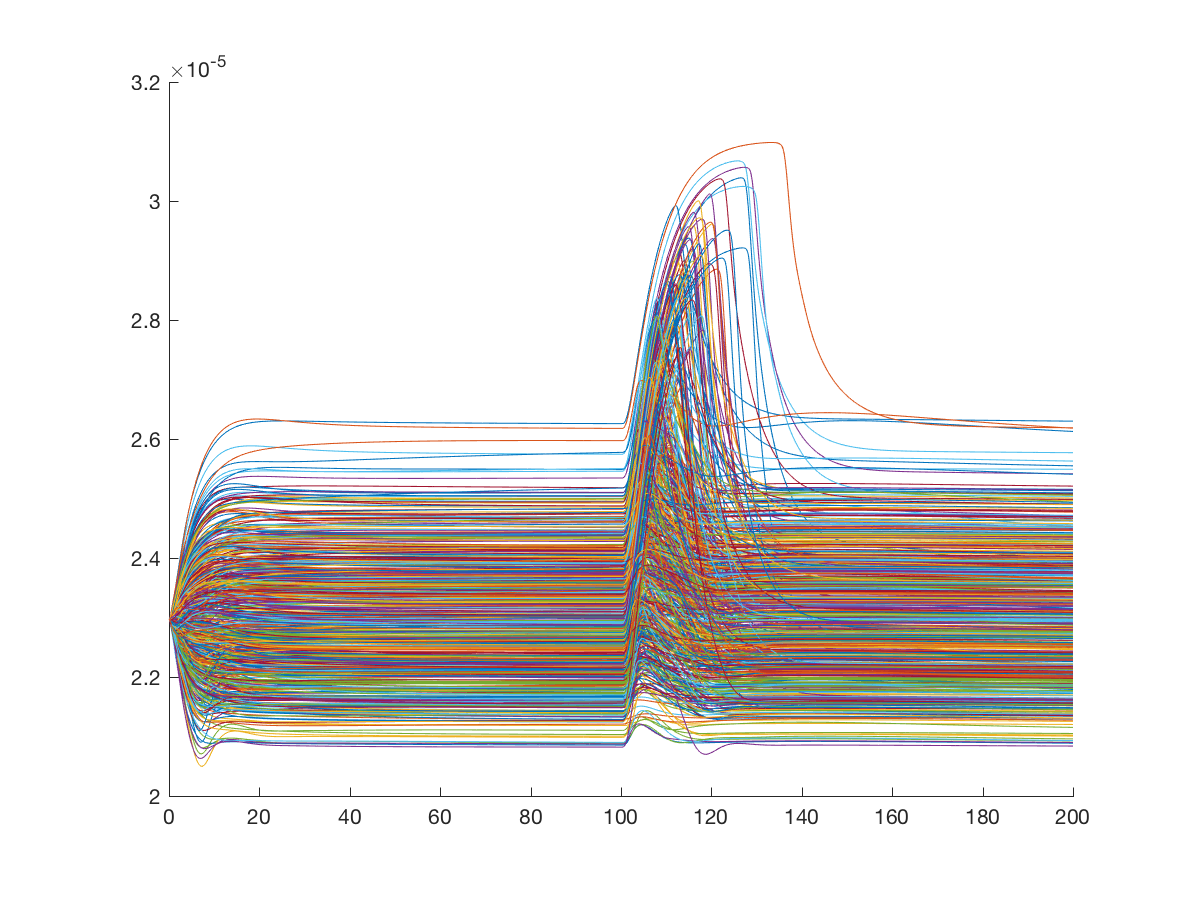
\includegraphics[width=.49 \textwidth]{Figures/Radius_Curves.eps}
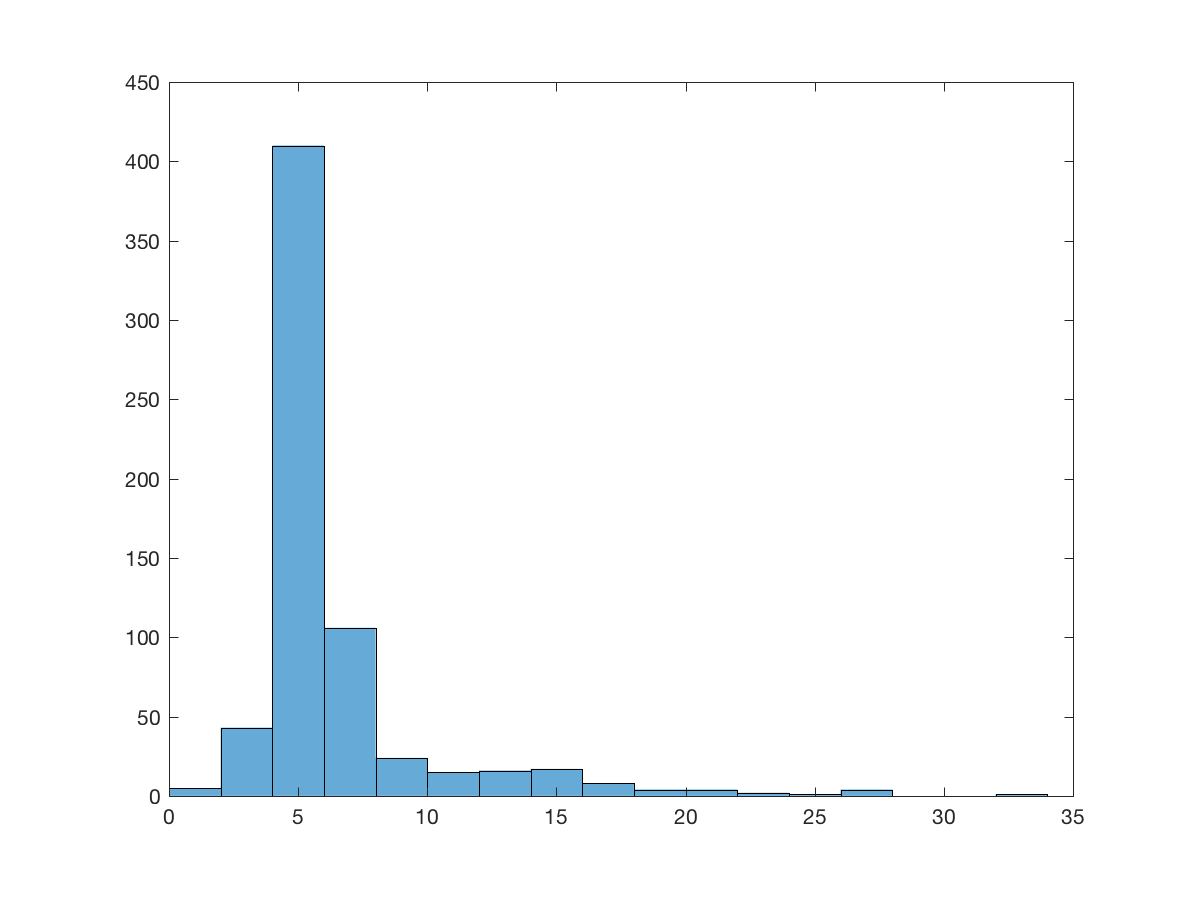
\includegraphics[width=.49 \textwidth]{Figures/Radius_Time_Lag_Histogram.eps}
\caption{Radius curves on the left and a histogram of the time lags on the right.}
\end{figure}
